\documentclass[a4paper]{article}

%% Language and font encodings
\usepackage[english]{babel}
\usepackage[utf8]{inputenc}
\usepackage{tabu}
\usepackage[T1]{fontenc}
\usepackage{enumitem}
\usepackage{amsmath}
\usepackage{xcolor}
\usepackage{amsfonts}
\usepackage{subfig}

%% Sets page size and margins
\usepackage[a4paper,top=3cm,bottom=2cm,left=3cm,right=3cm,marginparwidth=1.75cm]{geometry}
\usepackage{mathbbol}
\usepackage{sidecap}
\usepackage[format=plain, indention=1cm]{caption}


%% Useful packages
\usepackage{amsmath}
\usepackage{graphicx}
\usepackage{fancyhdr}
\usepackage{makecell}

\renewcommand\theadalign{bc}
\renewcommand\theadfont{\bfseries}
\renewcommand\theadgape{\Gape[4pt]}
\renewcommand\cellgape{\Gape[4pt]}
%% Title
\title{\textbf{Playing card detection}\\ PlayCDC\\Object recognition and image understanding lecture}
\author{Frank Gabel and Daniel Gonzalez}

\date{15.07.2018}

\begin{document}
\maketitle
\section{Abstract}
With the capabilities of upcoming small video capturing devices in, for example, smart contact lenses with built-in cameras, whole new ways of cheating in cardgames emerge. In order to help facilitate these cheating endeavours, we implement an algorithm that detects the suits and ranks of playing cards in the field of view of a camera using the latest iteration of the YOLO object recognition algorithm.
\begin{figure}[h]
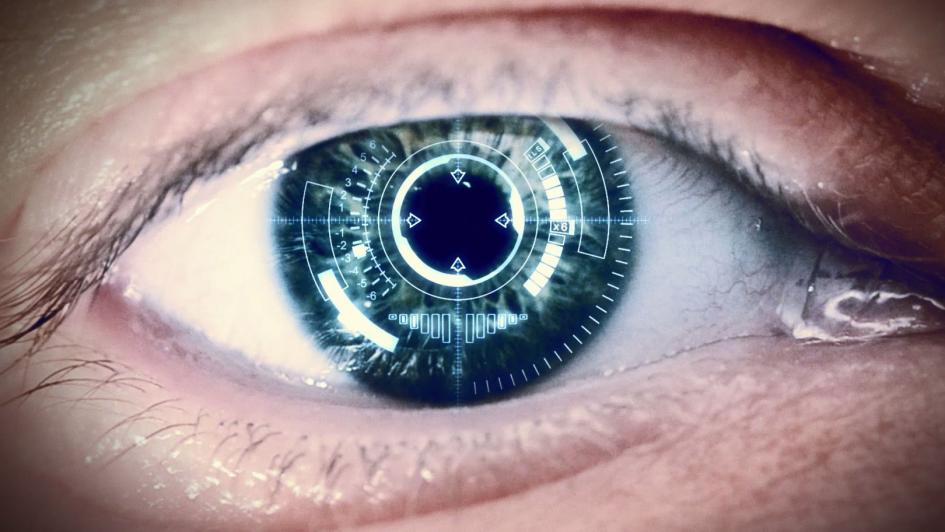
\includegraphics[scale=0.25]{contact_lense}
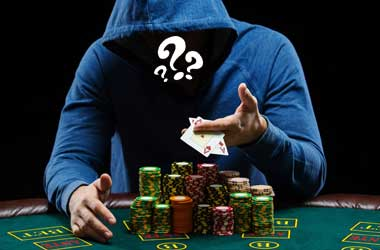
\includegraphics[scale=0.532]{poker_player}
\caption{Stock photos of an envisioned camera-equipped contact lense (left) and a mysterious black-jack player (right)}
\end{figure}
\section{Introduction}
A big topic in computer vision is the search of methods that are, given a query image, capable of answering questions like: What is present in an image? Is there a particular object in it? Where exactly in the image is this object located? Is it possible to semantically segment objects of interest in the image?
Object detection deals with detecting instances of semantic objects of a certain class (such as humans, buildings, or cars) in digital images and videos. Typically, object detection deals with two sub-taks: \textbf{object localization} using bounding boxes and \textbf{multiclass object classification} within said bounding boxes.
Sometimes, a third sub-task of \textbf{semantic object segmentation} is performed, i.e. the process of labelling objects on pixel level.\\
In this project, we use the YOLOv3 object detection algorithm (CITE) for object detection (without additional segmentation) in order to tell apart playing cards of a standard 52-part deck.

\section{Dataset}
The foundation of a machine learning project is based training on data in order to build a model that can recognize patterns.   For our detection model, we needed to have a large dataset of cards, together with the Boundy Boxes information for each of the cards logos.  Unfortunately, as there was no suitable dataset of cards available, we decided to create it by our own.  We did this in mainly two big steps, generating at the end 750 training images for each card, as well as the Bounding Box information necessary for the training step.   \\
The first necessarily step was to prepare the data in such a way, that it could be easily used later for data generation.  Here, it was important to detect the convex hulls of the card logos, because they were necessary to become the Bounding Boxes information.  The reason why we worked with convex hulls, instead of Bounding Boxes from the beginning on, will be explained in the later subsection.
The second big step was focused on generate new data.  For this, we applied linear transformations, as well as blurring, sharpening, change of lighting and rotation to the cards. 
For this, it was necessary to keep track of the convex hulls when applying the transformations. 

\subsection{Data preparation}
We decided to work with 50 cards of a deck of 52 cards, where each card contains two times its logo.  First, we took for each card 2 different photos, manually crop the cards to a selection and then rescale the result by 600x900 pixels.  We choose this resolution arbitrary, as we though that it was a good size to begin with.
In this step, we used the selection/rotation/cropping/rescale -tools provided by GIMP\footnote{GIMP 2.8.22 - GNU Image Manipulation Program}. \\
Concluding this, we proceed by detecting the convex hulls of the cards suits and ranks.   We used here the Python libraries SciPy\footnote{SciPy: Open Source Scientific Tools for Python} and OpenCV\footnote{OpenCV: Open Source Computer Vision Library} to detect in a semi-automatic way the regions and convex hulls of each of the two card logos (Figure \ref{fig-data-prep} illustrates this preceding).  After verifying the desired result for each card, we saved the two convex hulls of each card as an NumPy array. \\

%\begin{figure}[h]
%\centering
%\captionsetup[subfigure]{labelformat=empty}
%\subfloat[\scriptsize Queen of spades with a resolution of 600x900 pixels ] {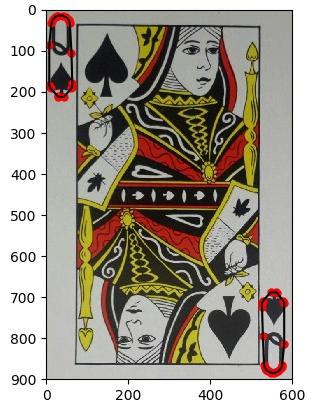
\includegraphics[scale=0.387]{qs_2}}  \hspace{2cm}
%\subfloat[\scriptsize Zoomed convex hulls.  The red points are saved.] {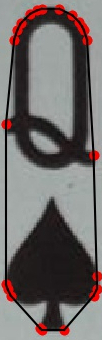
\includegraphics[scale=0.455]{qs_2_1} \quad
%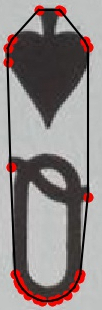
\includegraphics[scale=0.5]{qs_2_2} }
 %\caption{Stock photos of an envisioned camera-equipped contact lense (left) and a mysterious black-jack player (right)}
%\end{figure}
\begin{minipage}{\columnwidth}
\makeatletter
\newcommand{\@captype}{figure}
\makeatother
\centering
\captionsetup[subfigure]{labelformat=empty}
\subfloat[\scriptsize Queen of spades with a resolution of 600x900 pixels.]{%
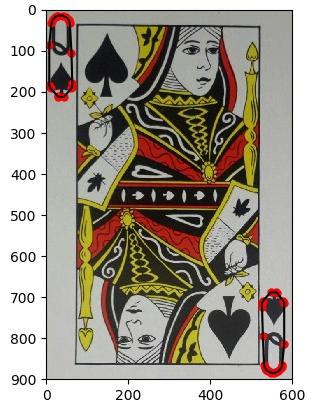
\includegraphics[scale=0.587]{qs_2}%
\label{fig:evaluation:revenue}}\qquad \qquad%
\subfloat[\scriptsize Zoomed convex hulls.  The red points were saved as a NumPy array.]{%
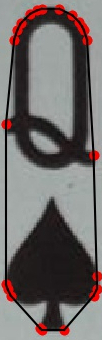
\includegraphics[scale=0.68]{qs_2_1} \quad
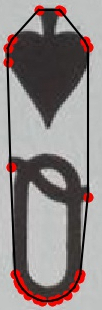
\includegraphics[scale=0.74]{qs_2_2}  }
\caption{Semi automatic detection of the convex hulls.}
\label{fig-data-prep}
\end{minipage}

\subsection{Synthesize a general dataset}
With all the images in the same resolution and having detected the Bounding Boxes for each card, the next goal was to generate a big amount of new data destined to train our model. 
First, we randomly blurred the cards using Gaussian, Average and Median filters.  We did also randomly perform sharping and lightning operations on the image.  After this, we pasted the cards in 3000x3000 pixels scaled canvases provided by DDT \cite{cimpoi14describing}.  The reason why we chose to work with such big canvases, will be more clear while reading this subsection.  Notice, that after pasting the images on the canvases, we had to translate the convex hulls to their new positions.\\
In total, we pasted each card in 75 different textures for the training dataset and in 15 different textures for the test dataset.  Figure \ref{fig-canvas} illustrate some examples and textures.

\begin{minipage}{\columnwidth}
\makeatletter
\newcommand{\@captype}{figure}
\makeatother
\centering
\captionsetup[subfigure]{labelformat=empty}
\subfloat[ ]{%
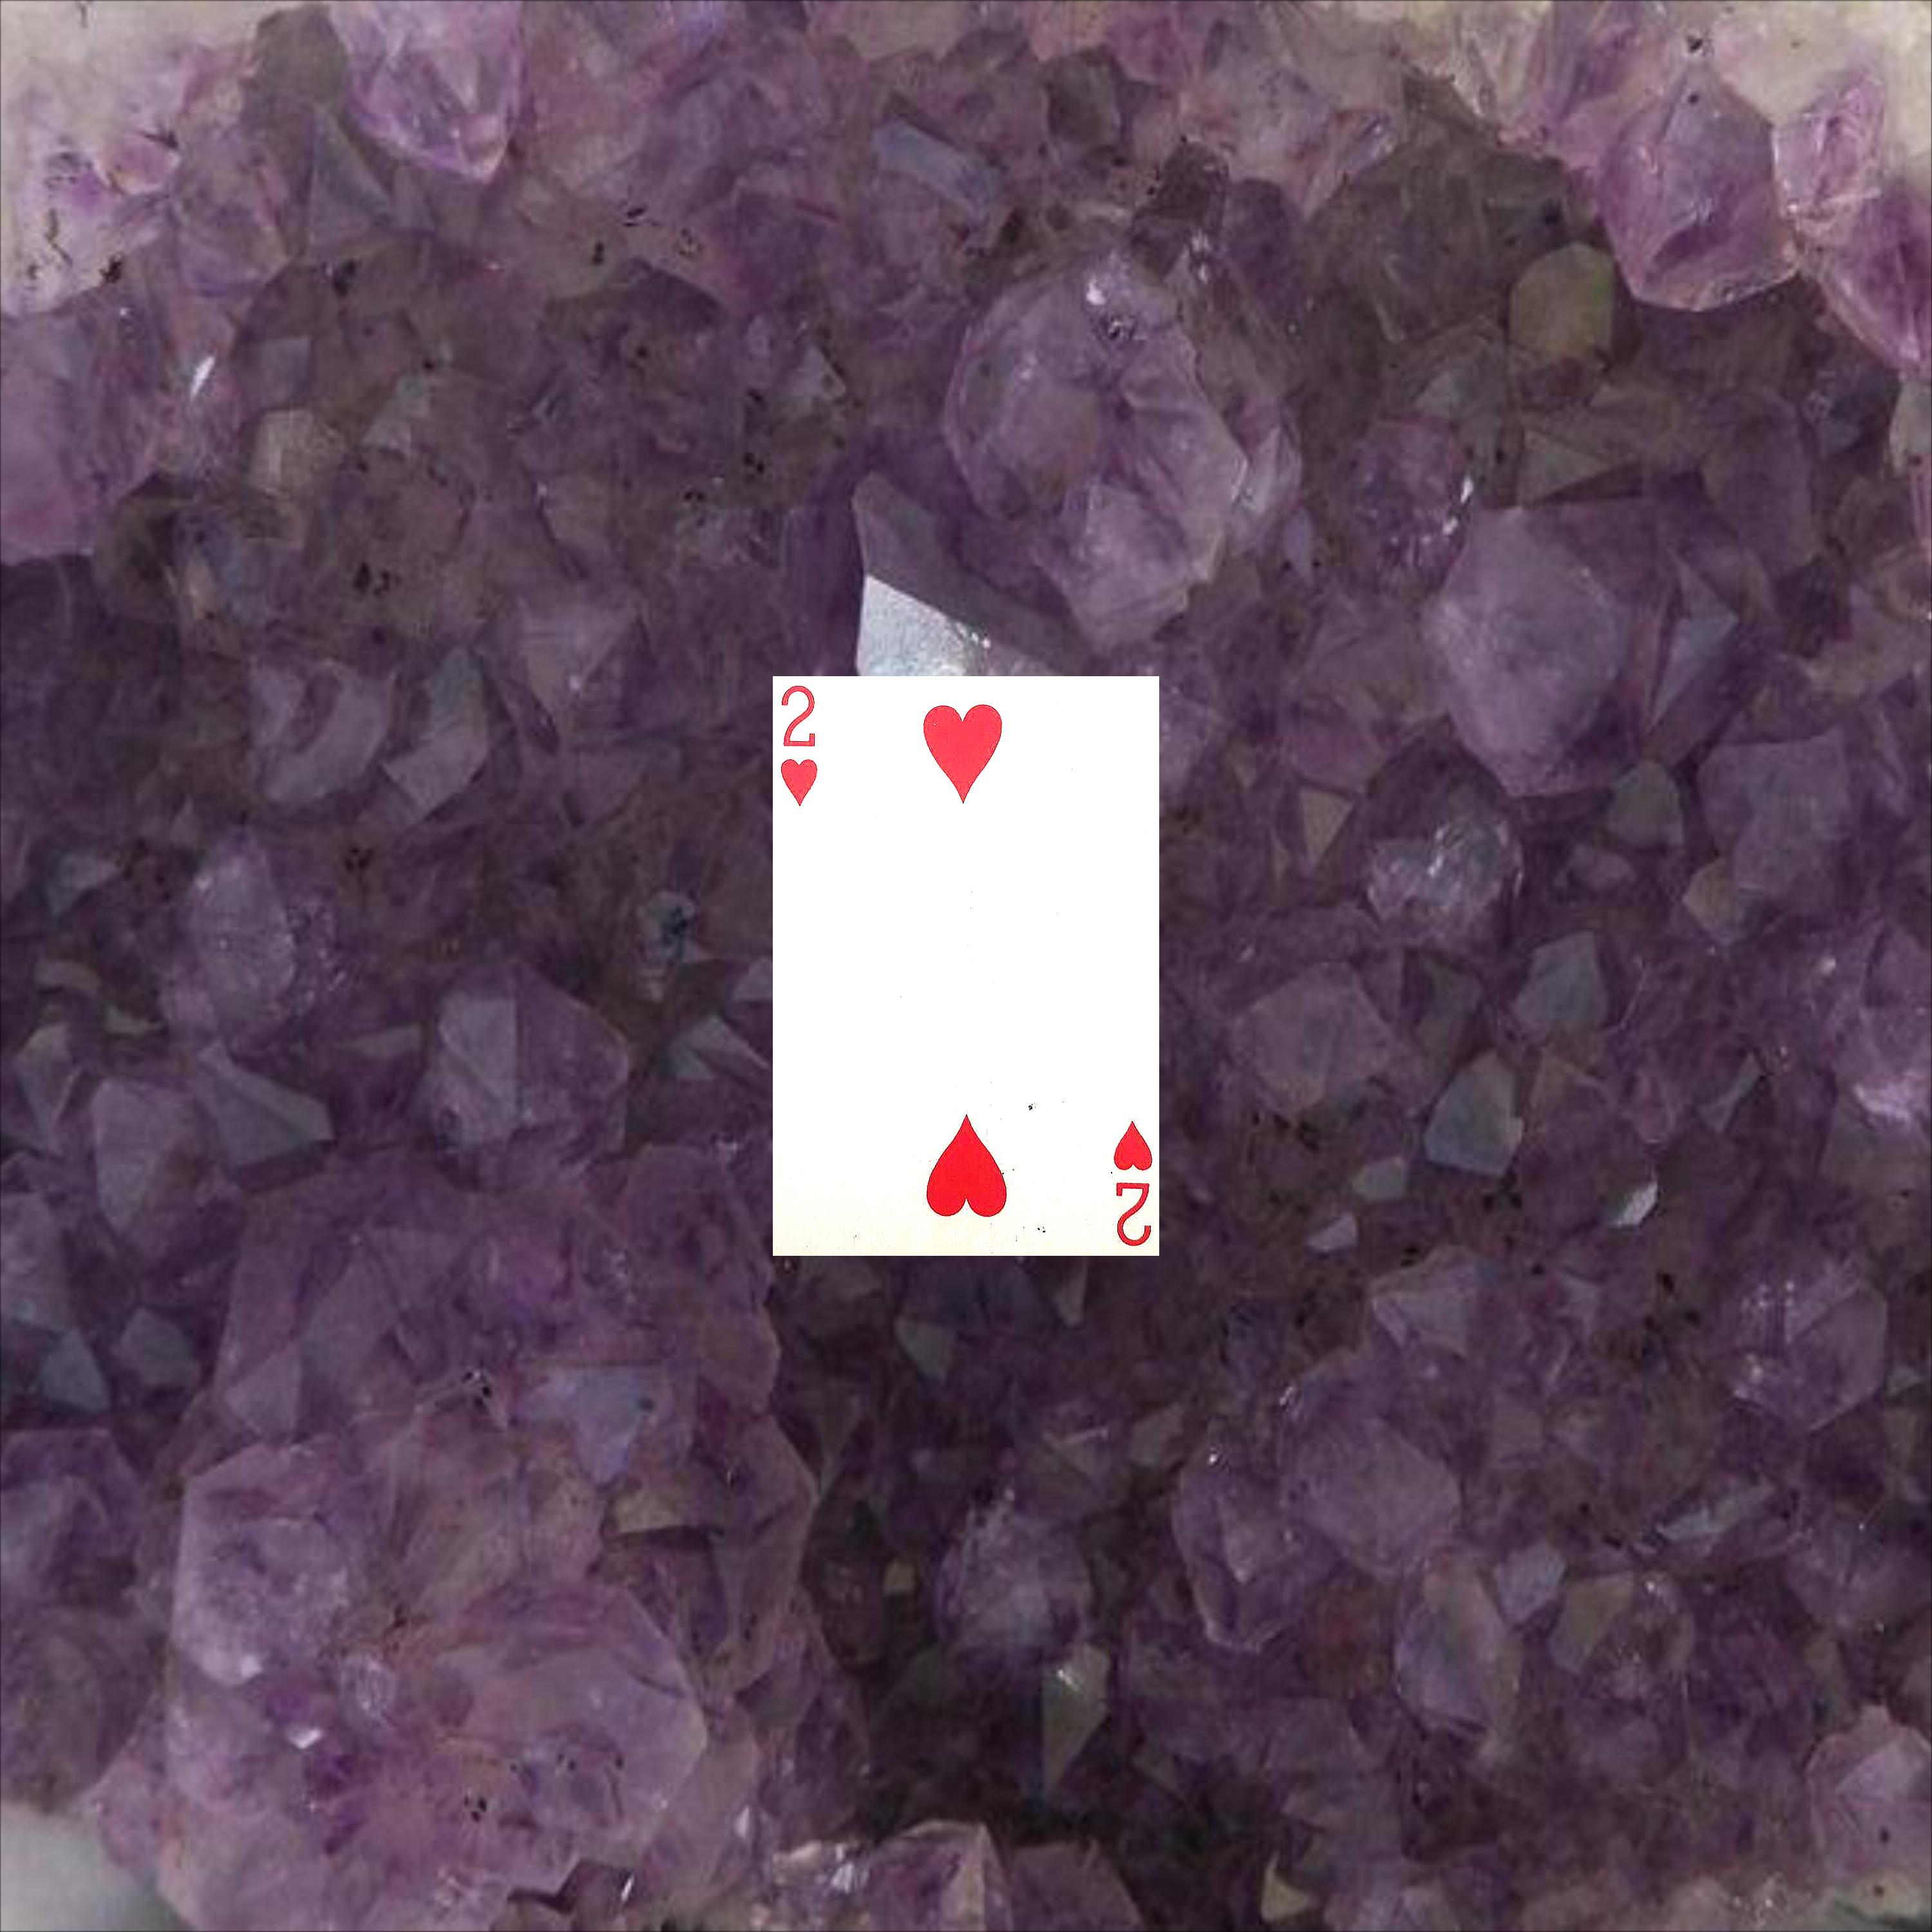
\includegraphics[scale=0.04]{2h_1}  \quad%  
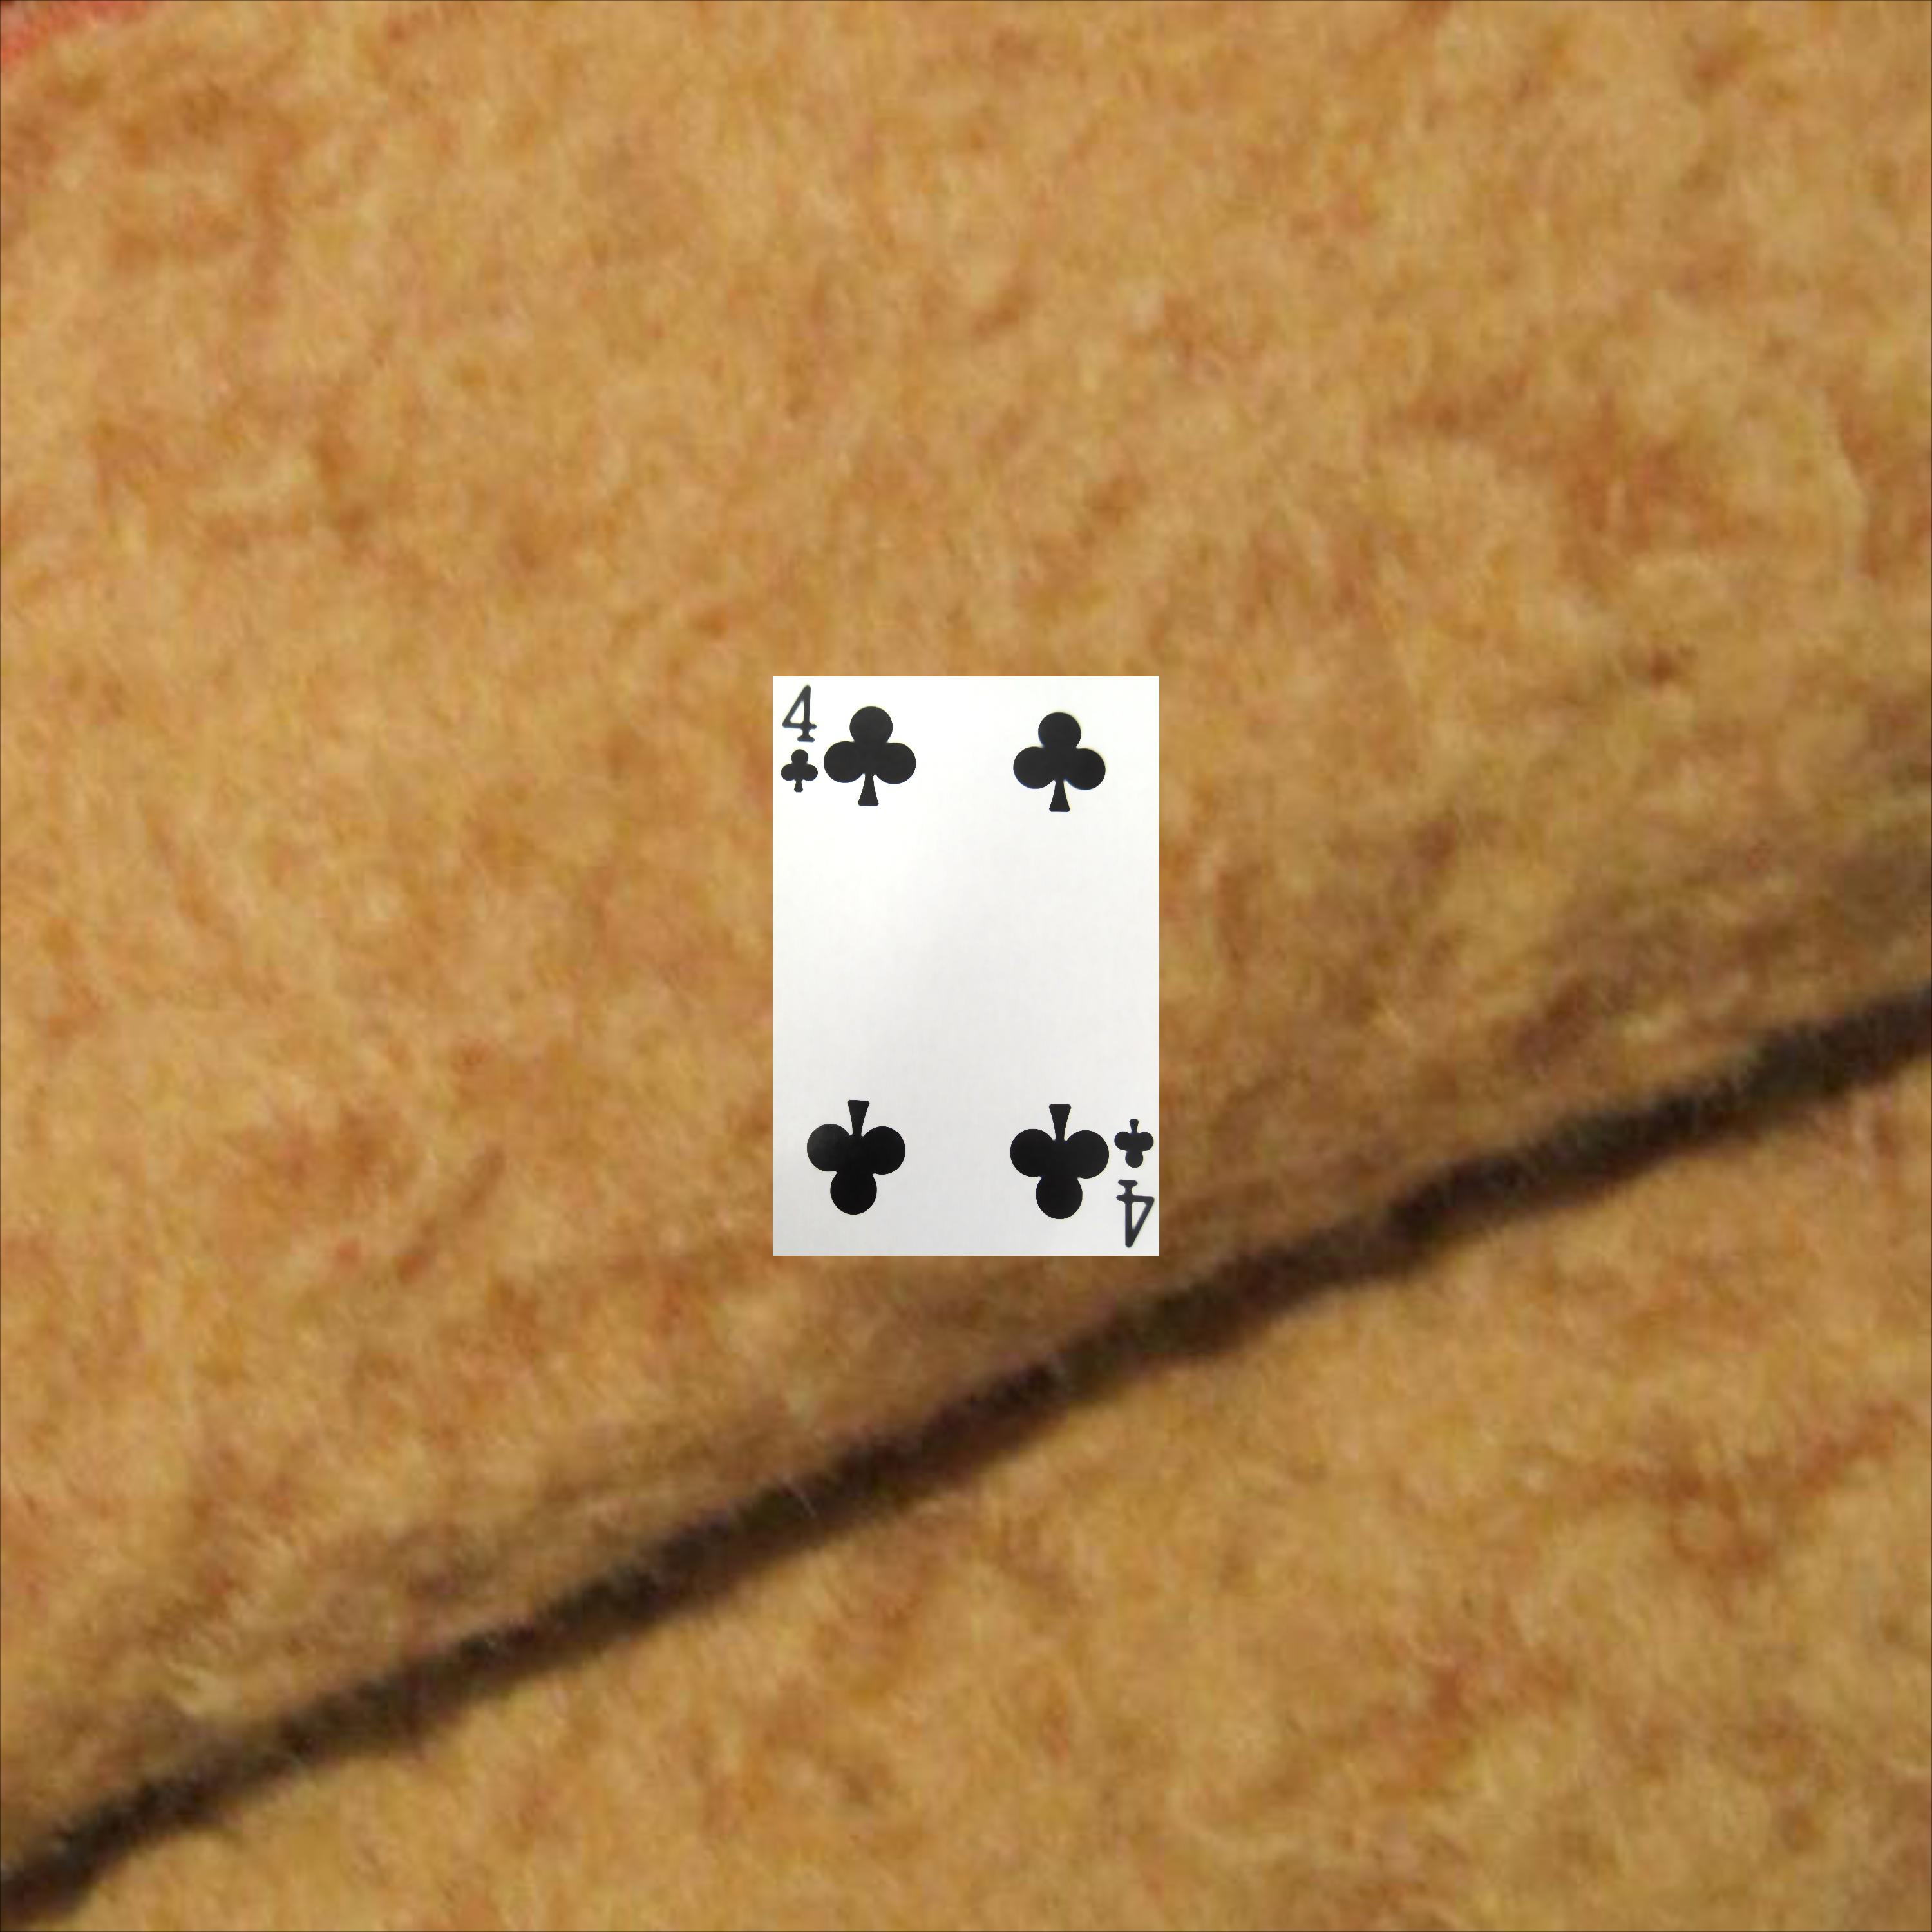
\includegraphics[scale=0.04]{4c_1}  \quad%  
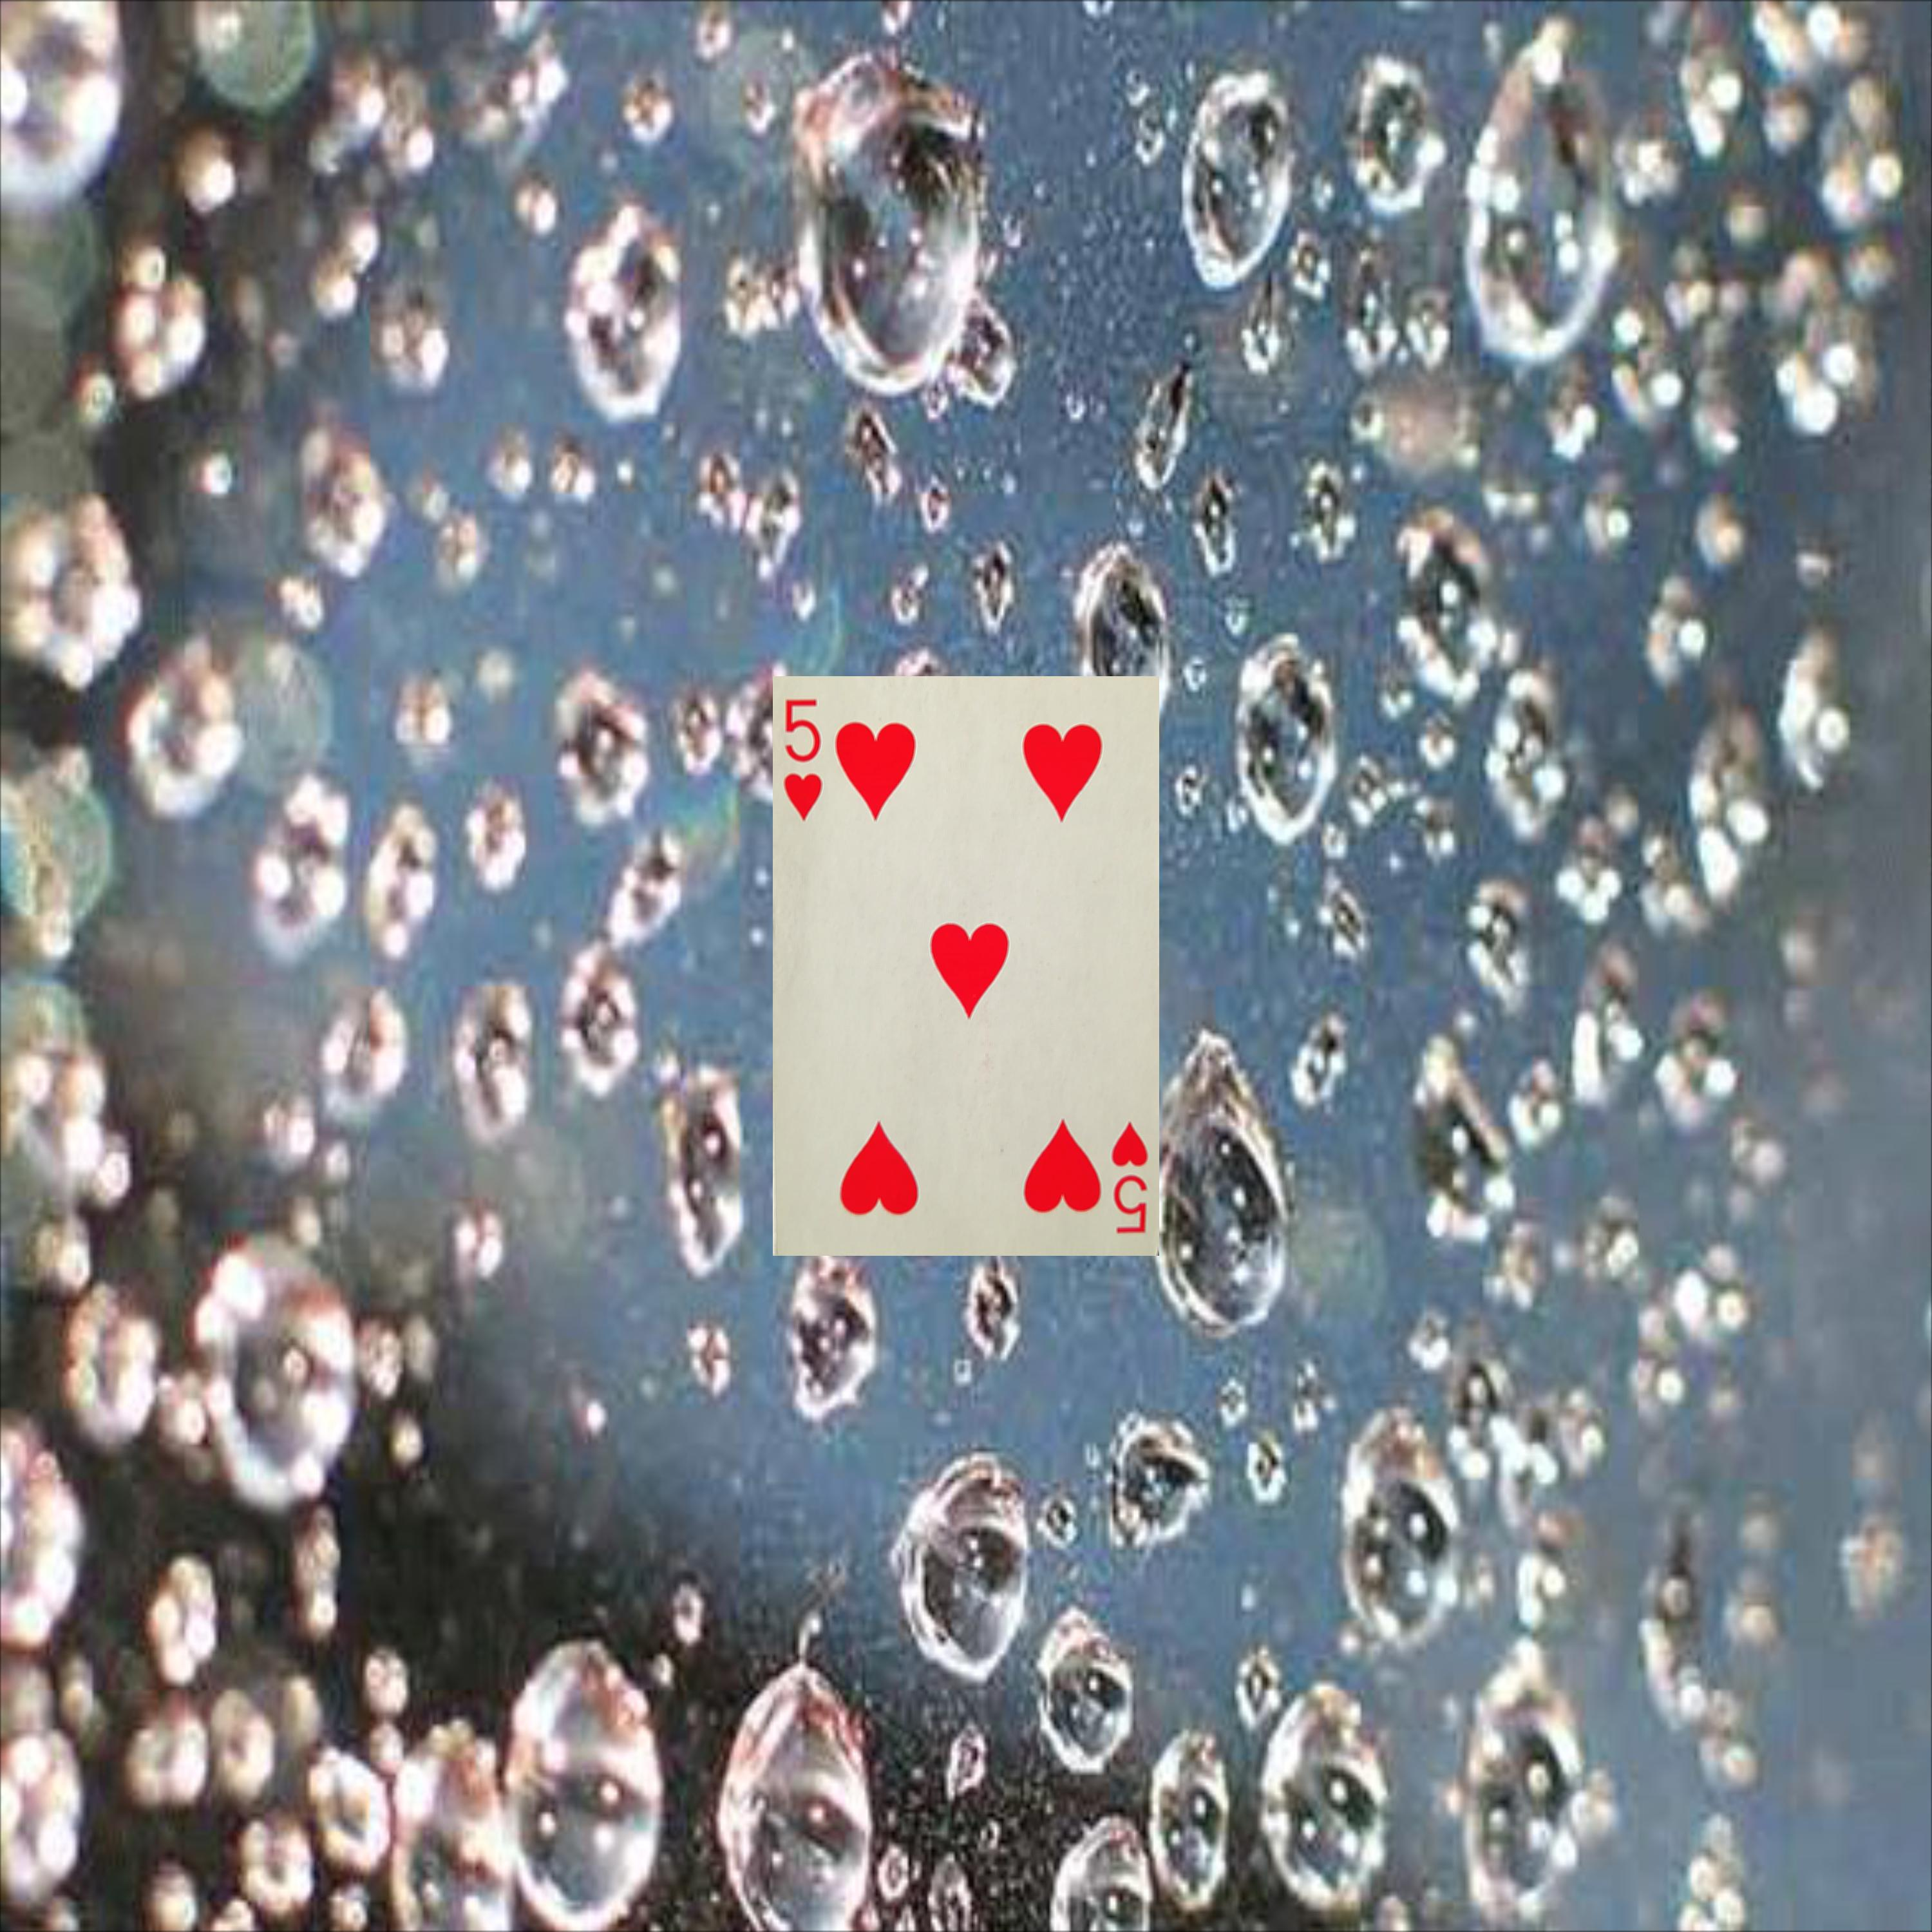
\includegraphics[scale=0.04]{5h_1}}  \qquad 
\subfloat{%
\vspace{1cm}
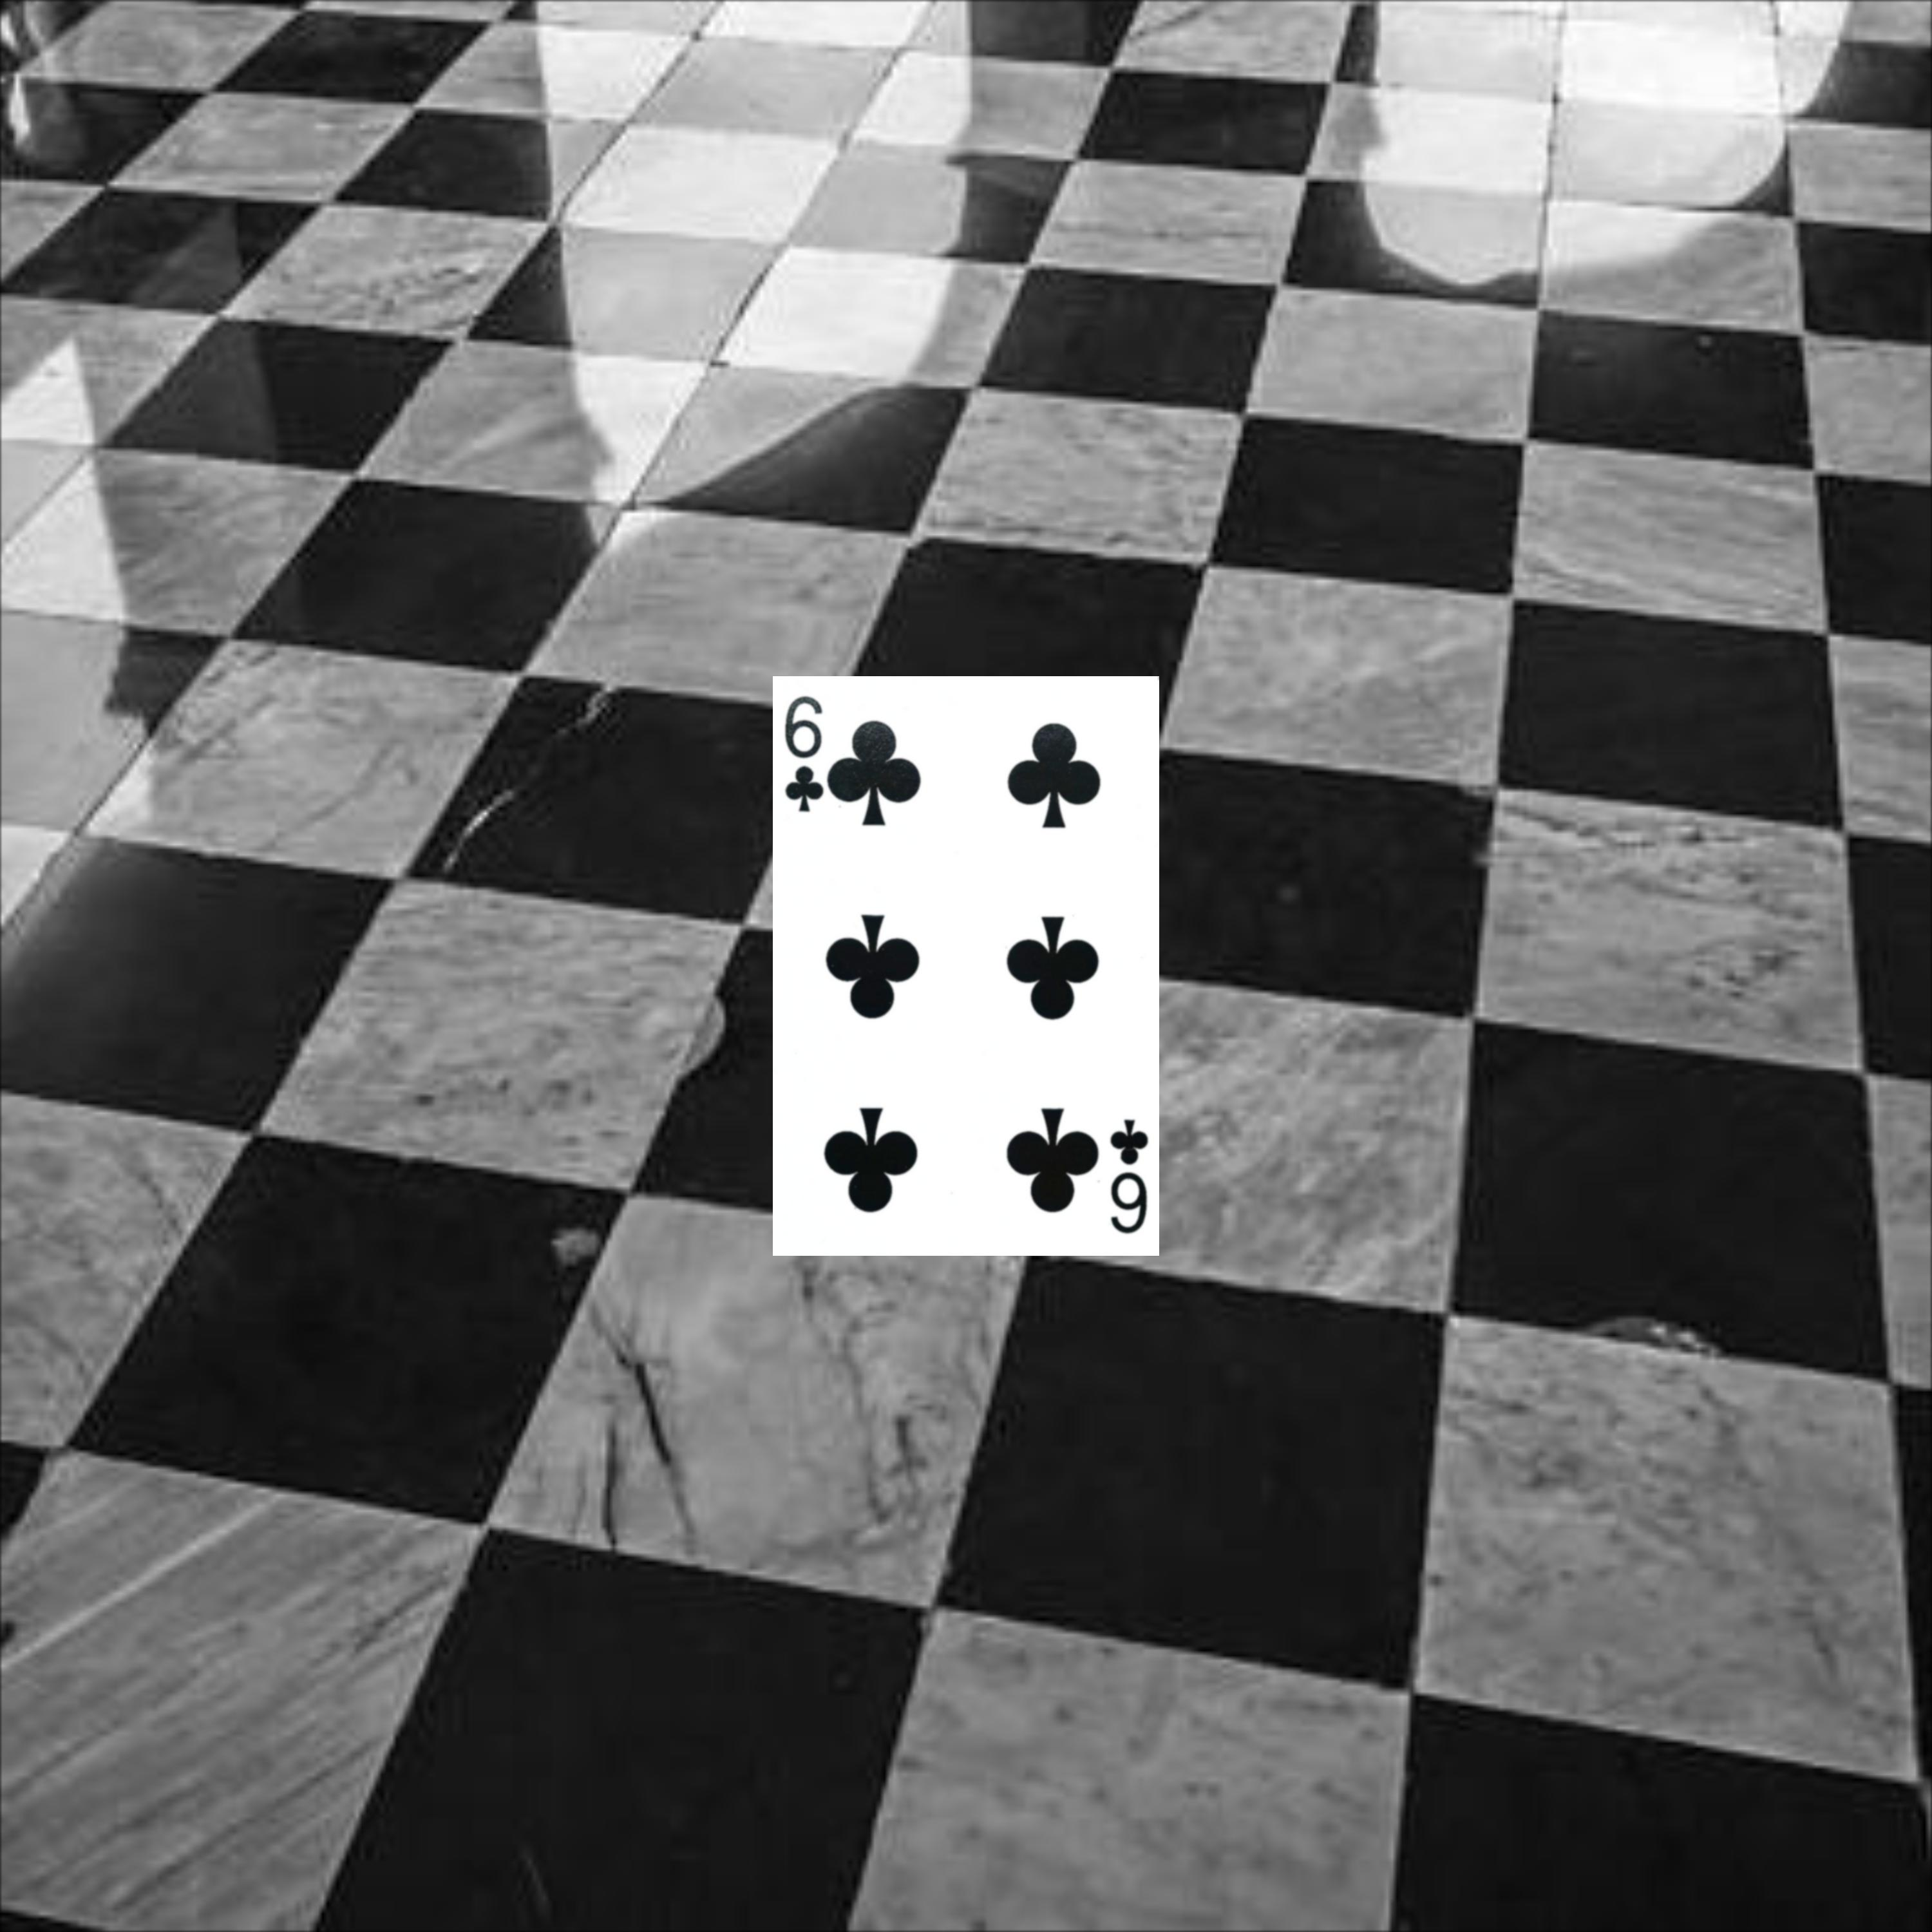
\includegraphics[scale=0.04]{6c_1}  \quad%  
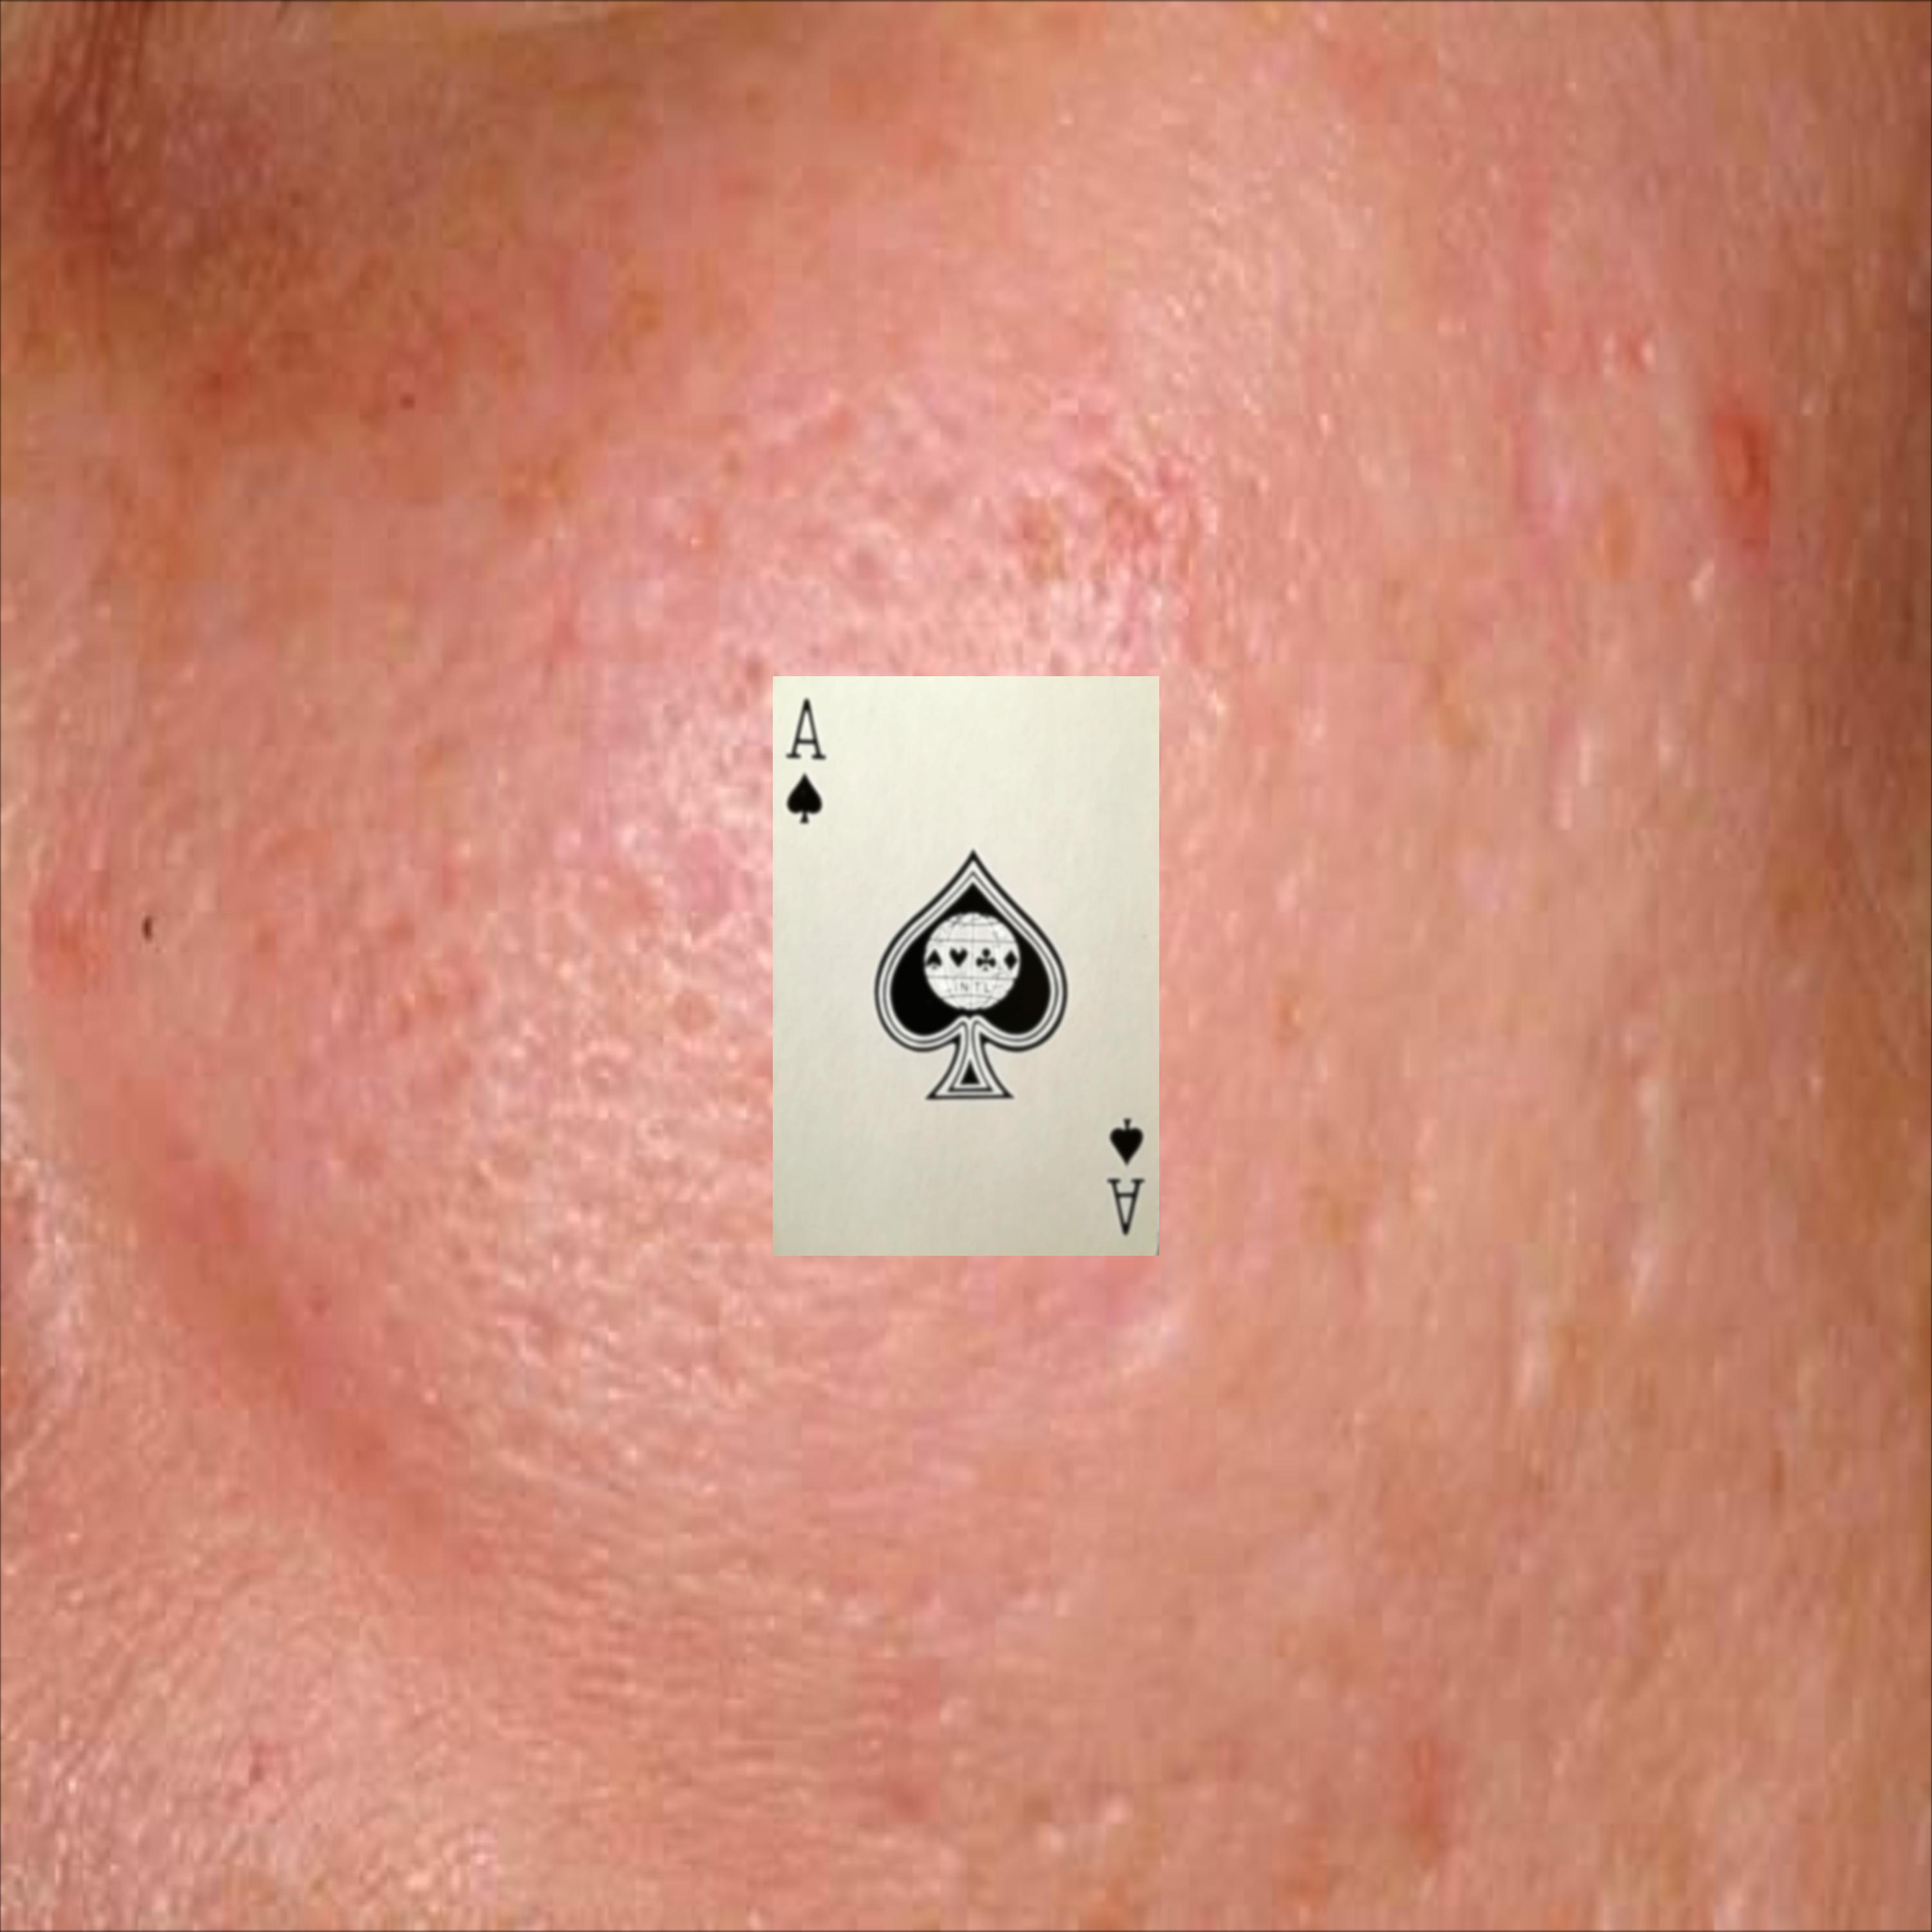
\includegraphics[scale=0.04]{as_1}  \quad
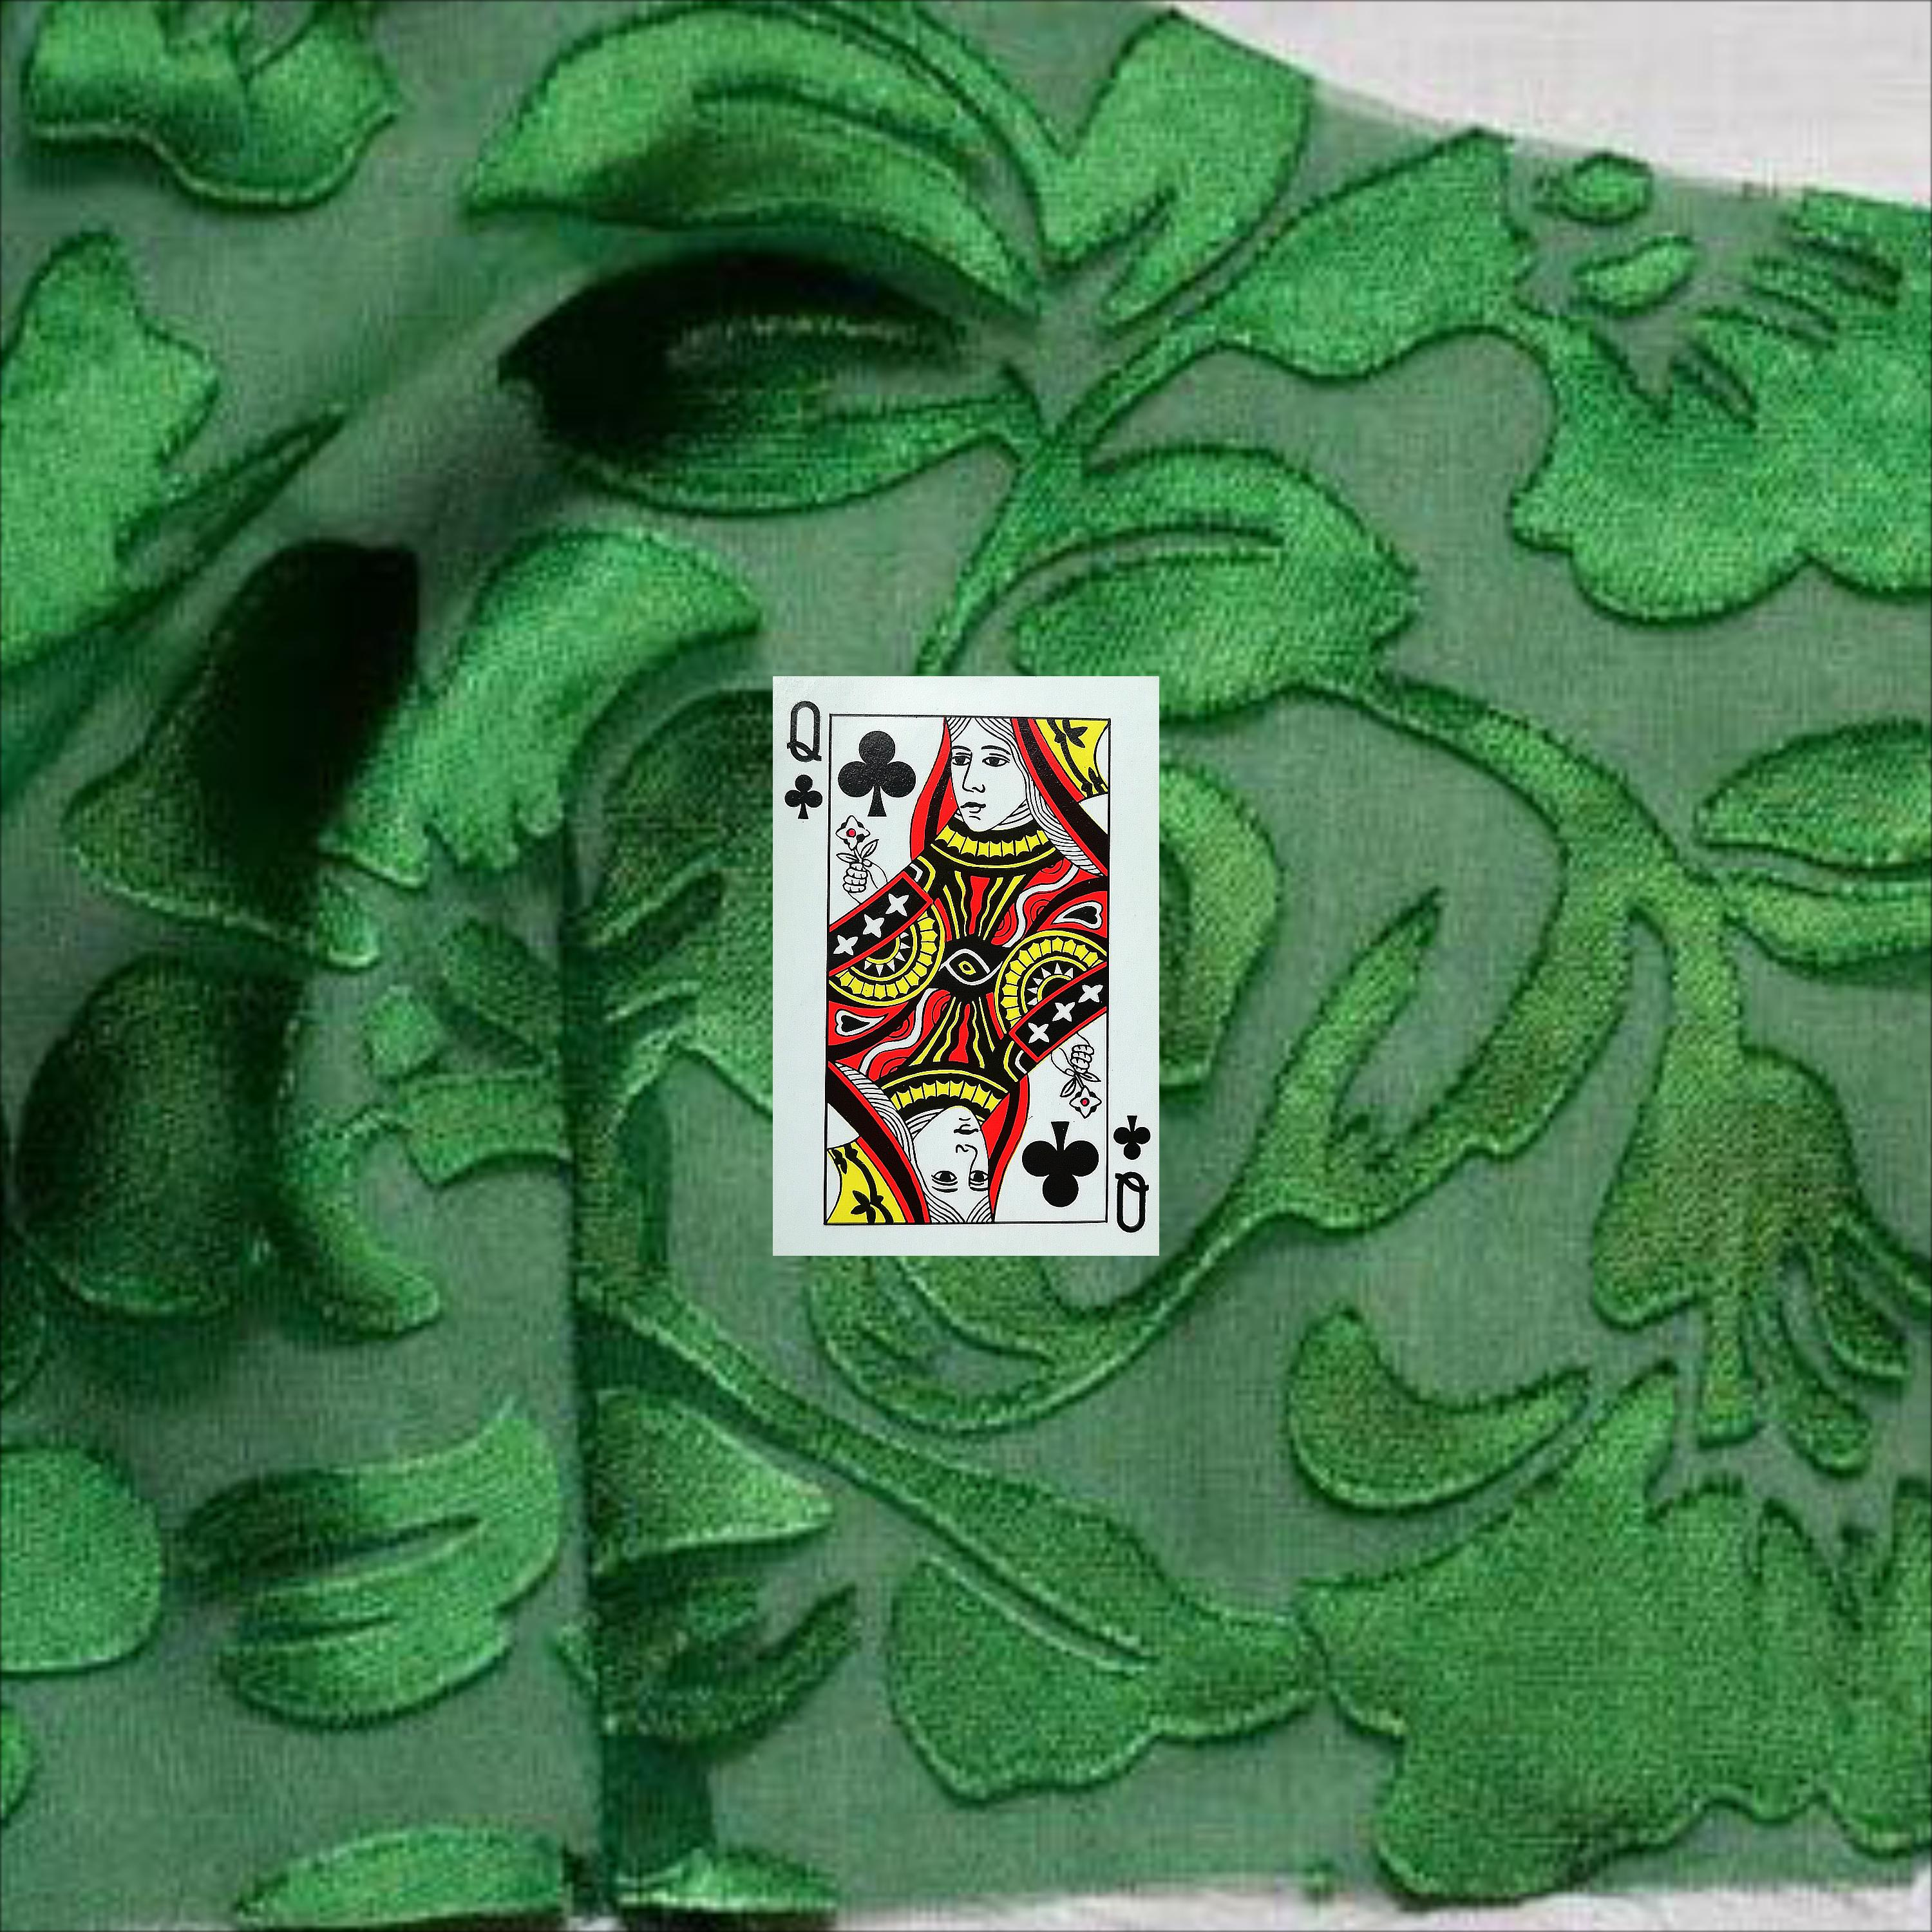
\includegraphics[scale=0.04]{qc_1} }
\caption{Some cards pasted into canvases of 3000x3000 pixels.}
\label{fig-canvas}
\end{minipage}
\newline \newline\newline 
\noindent The next step for the data generation was to perform a linear transformations on the image on canvas.  We randomly perform scaling, translation and rotation on the image using the imgaug python library.  After this, we crop the image reducing the pixel resolution by 800x800 pixels.  Notice that some of the convex hulls might be partially or complete lost when cropping.  This was with intention of making the dataset more realistic and fixed letting some boundary points take the role roll of the convex hulls (Compare this statement with the 5 of hearts in Figure \ref{img-cards examples}).   We also decided not to accept convex hulls with few points that were very near to the boundary.
Notice also, that having pasted the images on big canvases, allowed us to have a nice background after the rotation and cropping.\\
As mentioned before, we decided to use the imgaug python library, because it allowed us to keep track of the convex hulls while doing transformations.

\begin{minipage}{\columnwidth}
\makeatletter
\newcommand{\@captype}{figure}
\makeatother
\centering
\captionsetup[subfigure]{labelformat=empty}

\subfloat[]{%
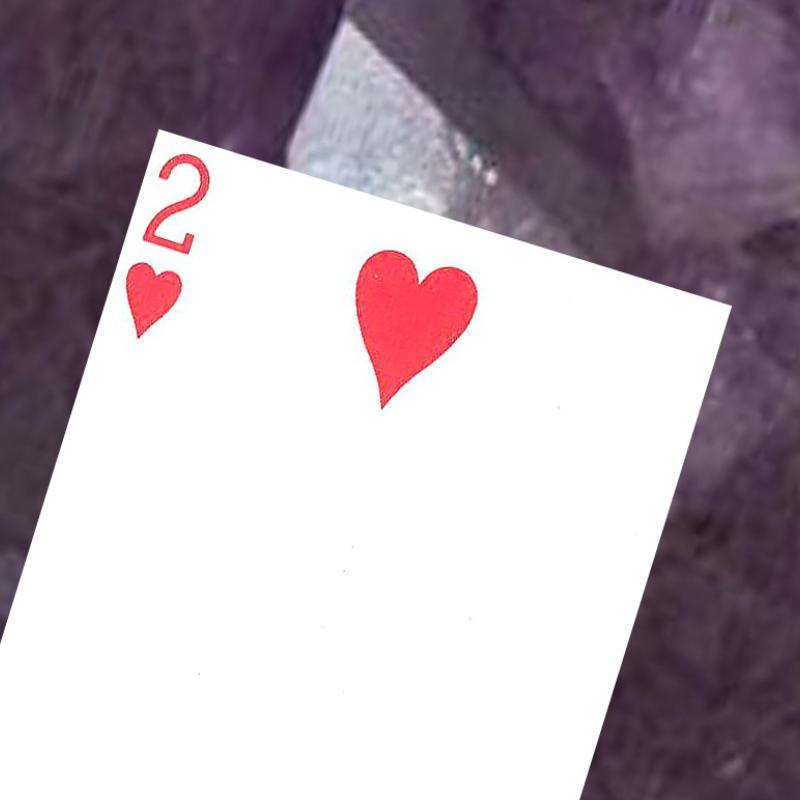
\includegraphics[scale=0.1125]{2h_2}  \ 
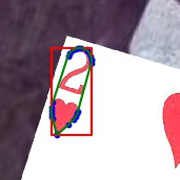
\includegraphics[scale=0.7]{2h_4}}  
\qquad
\subfloat{%
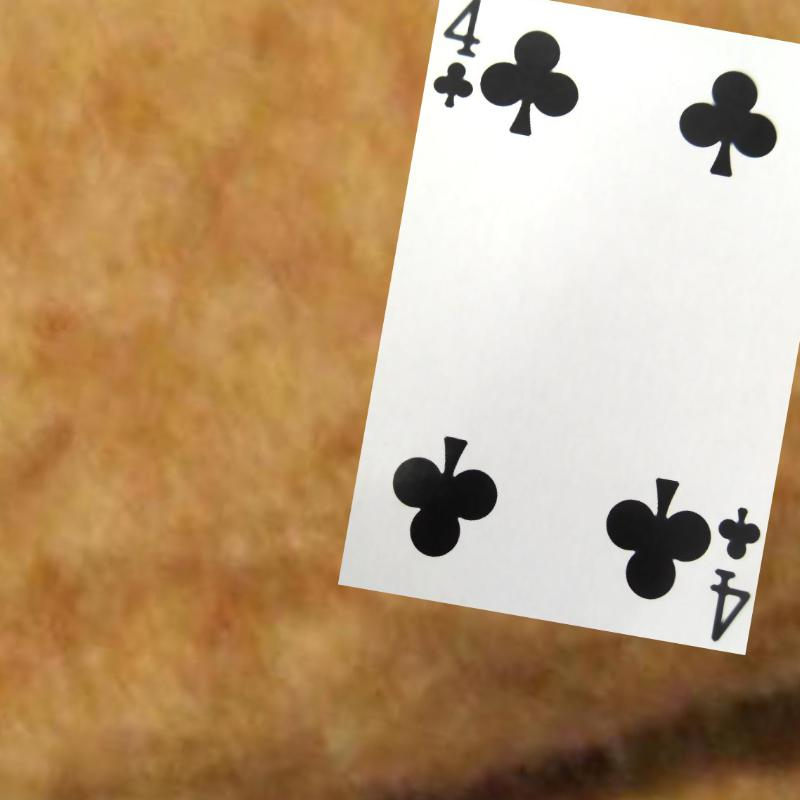
\includegraphics[scale=0.1125]{4c_2}  \  
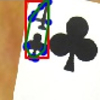
\includegraphics[scale=1.27]{4c_4}}  
\qquad
\subfloat{%
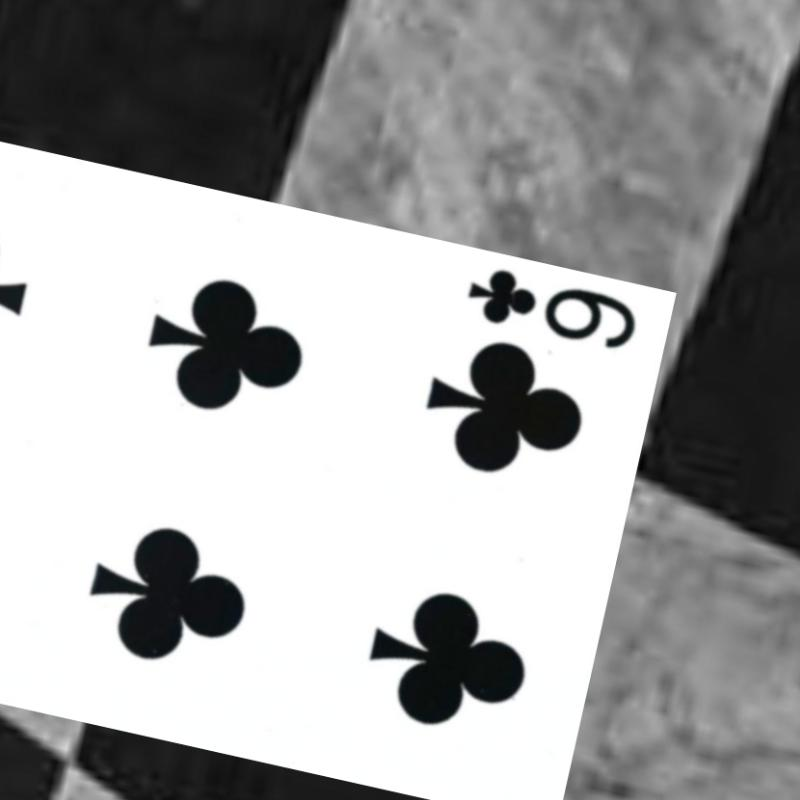
\includegraphics[scale=0.1125]{6c_2}  \
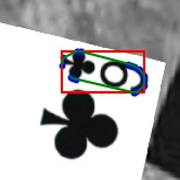
\includegraphics[scale=0.7]{6c_4}}  
\qquad
\subfloat[]{%
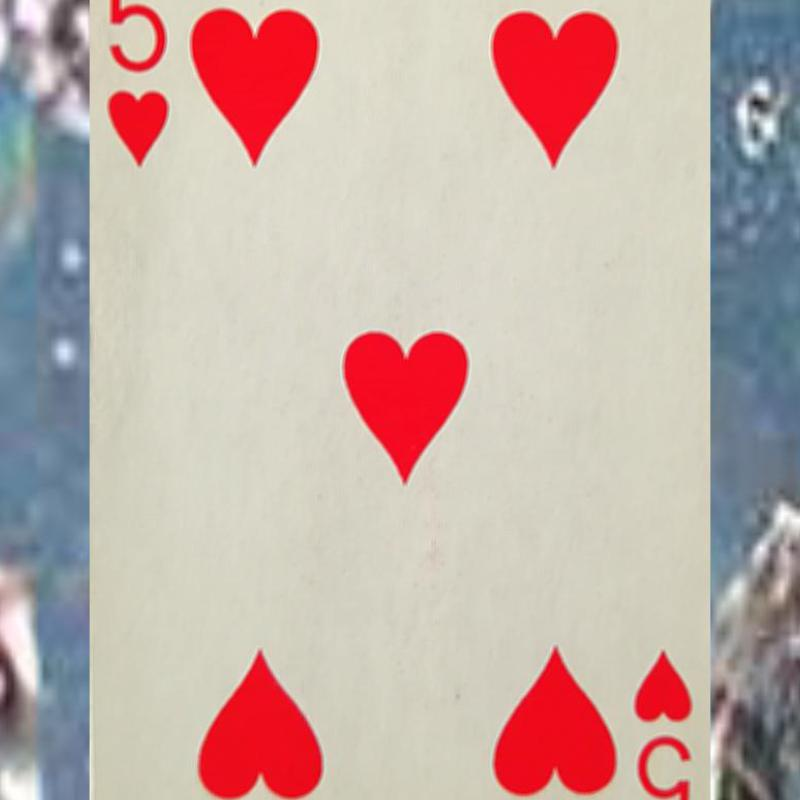
\includegraphics[scale=0.1125]{5h_2}  \
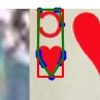
\includegraphics[scale=1.27]{5h_4}}  
\qquad
\subfloat{%
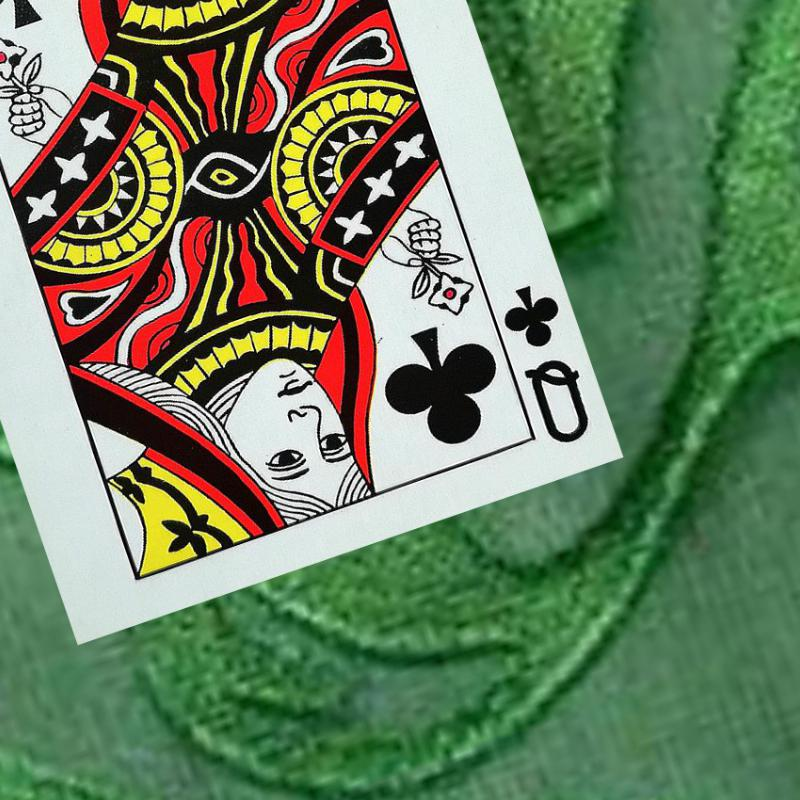
\includegraphics[scale=0.1125]{qc_2}  \
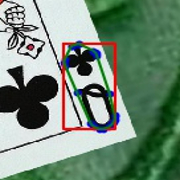
\includegraphics[scale=0.7]{qc_4}}  
\qquad
\subfloat{%
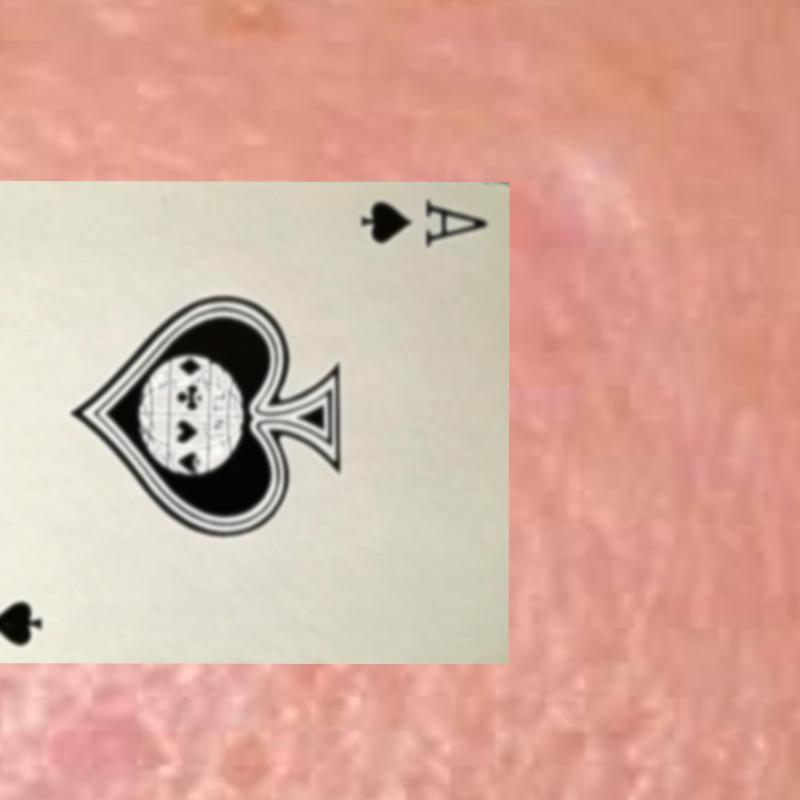
\includegraphics[scale=0.1125]{as_2}  \
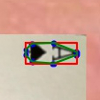
\includegraphics[scale=1.25]{as_4}}  
\qquad
\caption{Images of the previous paragraph after the mentioned transformations and cropping.  The right images are zoomed and contain the convex hulls as well as the final Bounding Boxes. }
\label{img-cards examples}
\end{minipage}

\subsection{The convex hull approach}
YOLOv3 expected for each image, a .txt file with a line for each ground truth object in the image that looks like:
<object-class><x><y><width><height>, where x, y are the center positions of the Bounding Boxes (BBs) and the width and height, also of the BBs, are relative to the image's width and height. \\
As mentioned before, we decided to work with convex hulls instead BBs from the beginning on.  The reason for this, is that otherwise we might have to increase the size of the BBs when doing rotations. Figure \ref{bb-ch} illustrates this problem.   Working with convex hulls on the other hand,  allowed us to obtain minimal BBs of the logos after applying transformations.

\begin{minipage}{\columnwidth}
\makeatletter
\newcommand{\@captype}{figure}
\makeatother
\centering
\captionsetup[subfigure]{labelformat=empty}
\subfloat[]{%
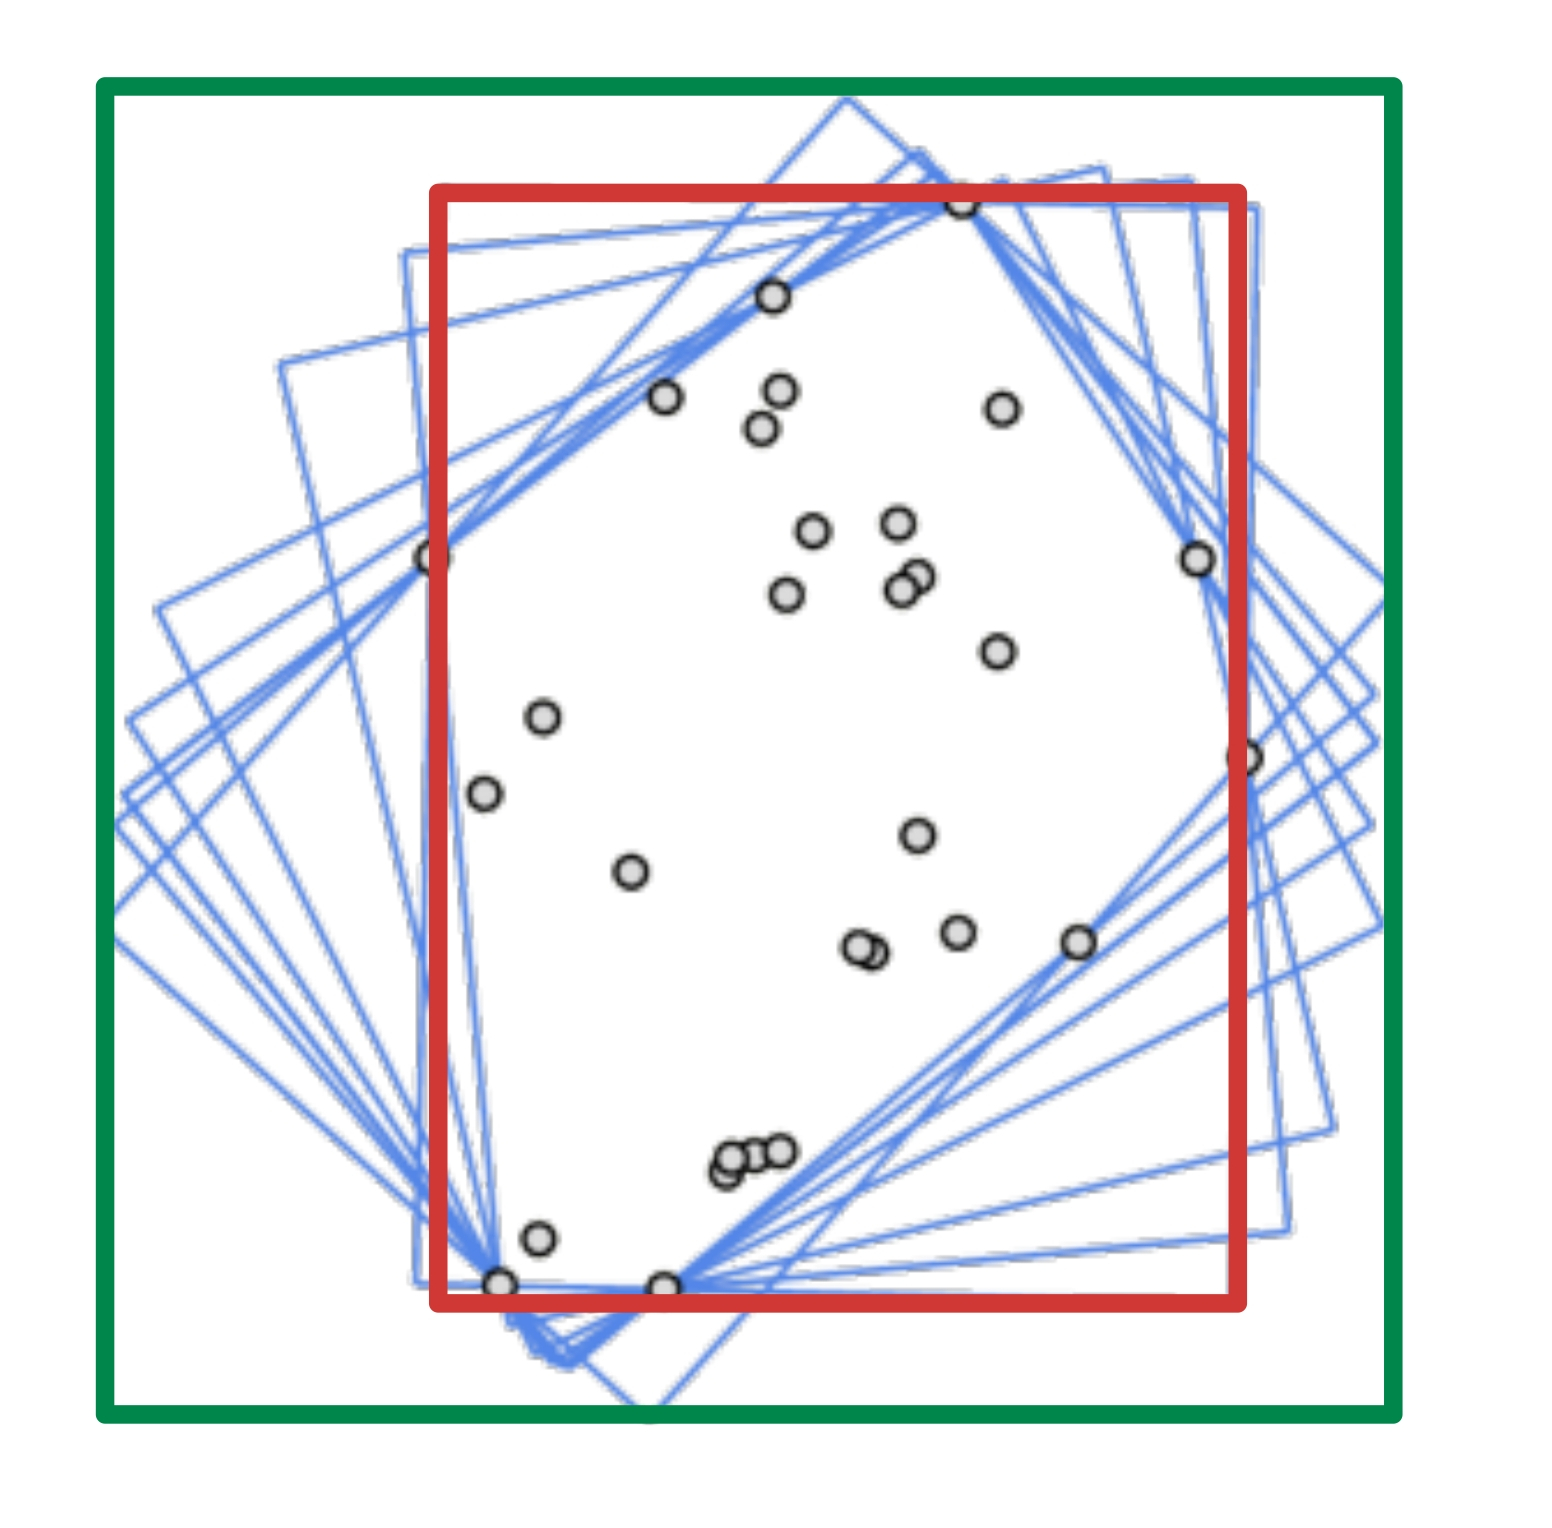
\includegraphics[scale=0.17]{ch_vs_bb}  }
\caption{Green box represents the BB when applying some rotations, while the red box represents the BB of the convex hull}
\label{bb-ch}
\end{minipage}




\section{Related work - The object detection landscape}
The task of object detection in images encompasses both the ``simpler'' form of only localizing and subsequently classifying objects as well as the more ``advanced'' form of additionally segmenting objects pixel-wise. For these tasks, different deep learning architectures have emerged, of which we will present the most important ones in the following.\\ In 2015, \textbf{Faster Region-based Convolutional Networks (Faster R-CNNs)} (CITE) have come up as an enhancement of the existing R-CNN and Fast R-CNN methods that are based on both region proposal networks to find candidate bounding boxes and detection networks to perform classification. Faster R-CNN extend this by introducing weight sharing of the convolutional features between region proposal network and detection network, facilitating nearly cost-free region proposals. 

\textbf{You Only Look Once (YOLO)}
\textbf{Single-Shot Detector (SSD)}
One-stage detectors like YOLO or SSD that are applied over a regular, dense sampling of possible object locations have the potential to be faster and simpler, but have trailed the accuracy of two-stage detectors because of extreme class imbalance encountered during training.
In \textbf{Focal Loss for Dense Object Detection (RetinaNet)}, researchers from FAIR therefore have developed a concept circumventing this - the idea is to reshape cross entropy loss such that it down-weights the loss assigned to well-classified examples. The novel focal loss focuses training on a sparse set of hard examples and prevents the vast number of easy negatives from overwhelming the detector during training. 



For sake of completeness, The \textbf{Mask Region-based Convolutional Network (Mask R-CNN)} consitutes the current state-of-the-art in semantic object segmentation. The basic idea is to.....
As this extends the scope of our project, we will not dive deeper and rather refer interested readers to the orginal research paper (CITE) or ...
\section{Methods}
\subsection*{The YOLO approach to object detection}
The YOLO model’s novel motivation is that it re-frames
object detection as a single regression problem, directly
from image pixels to bounding box coordinates and class
probabilities. This means that the YOLO model only ”looks
once” at an image for object detection.
It works as follows: 
\begin{itemize}
\item[--] divide an image into an $S\times S$ grid
\item[--]  predicts $B$ bounding boxes and a confidence score for each box (often called \textit{objectness score}) as well as a single $C$-dimensional vector of class probabilities
\item[--]  the output vector $S \times S \times (B\times 5 +C)$-dimensional
\end{itemize} The confidence scores show how confident the
model is that there is an object in that bounding box. At test time the conditional class probabilities and the individual box confidence predictions are multiplied, resulting in a feature map of bounding boxes "weighted" by their per-class confidence scores.
\begin{SCfigure}

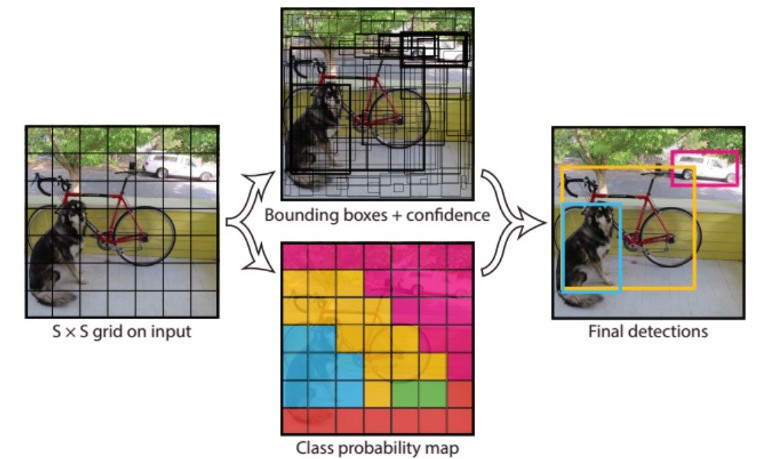
\includegraphics[scale=0.35]{yolo_model}

\caption{For each of the $S^2$ grid cells, we make one objectness prediction and four positional predictions for bounding boxes relative to each of the $B$ anchor boxes as well as a global class prediction vector. Combination of these values using NMS grants the final predictions.}


\end{SCfigure}


\subsubsection*{Anchor boxes}
Instead of wildly predicting $B$ bounding boxes per grid cell, the idea of YOLO is to predict offsets to $B$ so-called anchor boxes. Anchor boxes are pre-defined rectangular boxes that should be representative of as many ground-truth bounding boxes as possible.
\begin{SCfigure}
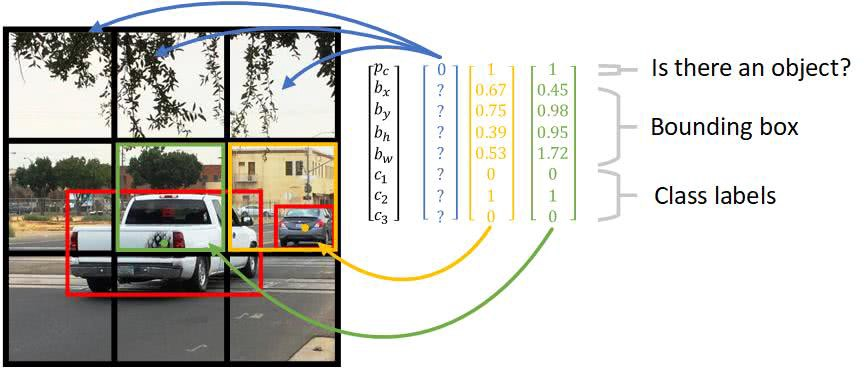
\includegraphics[scale=0.35]{yolo_mechanics}
\caption{For each grid cell, we predict vectors of multiple bounding boxes (here, only one bounding box is predicted, $B=1$), but only one class prediction vector of length $C$ (here, $C$=3).}

\end{SCfigure}
Confidence is formally defined as $P(Object) \times \text{IOU}^{pred}_{truth}$

. So its not something that model learns but something that you have to do up front. Look at the shape of bounding boxes in training data and separate then (maybe using some sort of clustering) and move those boxes to correct anchorbox (part of array) of training data.
YOLO is implemented as a 32 layer deep convolutional
neural network (DNN). The open source implementation released
along with the paper is built upon a custom DNN
framework written by YOLO’s authors, called darknet 1
.
This application provides the baseline by which we compare
our implementation of YOLO 2
. Redmon et al. have
released several variants of YOLO. For our purposes, we
chose the variant "tiny YOLOv3" which is a simplified version of YOLOv3 for restricted environments such as ours.\footnote{https://github.com/pjreddie/darknet/blob/master/cfg/yolov3-tiny.cfg}. In places in which the paper lacks details, we refer to the baseline darknet implementation
to resolve ambiguities.
\subsubsection*{Loss function}
YOLO’s loss function must simultaneously solve the object detection and object classification tasks. This function
simultaneously penalizes incorrect object detections
as well as considers what the best possible classification
would be. We employ the stochastic gradient descent
optimization method offered by TensorFlow[10] with the
Adam optimizer [7] to minimize the cost function. We
implement the following loss function, composed of five
terms:
\begin{align*}
\lambda_\textbf{coord}
\sum_{i = 0}^{S^2}
    \sum_{j = 0}^{B}
     {\mathbb{1}}_{ij}^{\text{obj}}
            \left[
            \left(
                x_i - \hat{x}_i
            \right)^2 +
            \left(
                y_i - \hat{y}_i
            \right)^2
            \right]&\textbf{\ coordinate loss}
\\\\
+ \lambda_\textbf{coord} 
\sum_{i = 0}^{S^2}
    \sum_{j = 0}^{B}
         {\mathbb{1}}_{ij}^{\text{obj}}
         \left[
        \left(
            \sqrt{w_i} - \sqrt{\hat{w}_i}
        \right)^2 +
        \left(
            \sqrt{h_i} - \sqrt{\hat{h}_i}
        \right)^2
        \right]\\
+ \sum_{i = 0}^{S^2}
    \sum_{j = 0}^{B}
        {\mathbb{1}}_{ij}^{\text{obj}}
        \left(
            C_i - \hat{C}_i
        \right)^2&\textbf{\ objectness loss}
\\
+ \lambda_\textrm{noobj}
\sum_{i = 0}^{S^2}
    \sum_{j = 0}^{B}
    {\mathbb{1}}_{ij}^{\text{noobj}}
        \left(
            C_i - \hat{C}_i
        \right)^2\\ 
+ \sum_{i = 0}^{S^2}
{{1}}_i^{\text{obj}}
    \sum_{c \in \textrm{classes}}
        \left(
            p_i(c) - \hat{p}_i(c)
        \right)^2&\textbf{\ classification loss}
\end{align*}


\subsubsection*{techniques}
\begin{description}
\item[Non-max suppression] Non max suppression removes the low probability bounding boxes which are very close to a high probability bounding boxes.
\end{description}

\subsubsection*{tiny YOLO-v3}

The particular architecture we used for training on our dataset is \textbf{tiny YOLOv3} which essentially is a smaller version of YOLO for constrained environments.
\begin{figure}


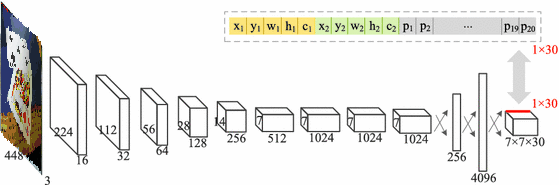
\includegraphics[width=1\linewidth]{tinyyolo}
\caption{tiny YOLO-v3 feature extractor}
\end{figure}

\subsection{Webcam deployment}
LETS PUT A PHOTO OF A LAPTOP WITH OUR STUFF RUNNING?
\subsection{Evaluation}
Each model is judged by its performance over the validation dataset. For each application, it is critical to find a metric that can be used to objectively compare models.
In Object detection in particular, it is crucial to measure how well the detection and classification was performed.  
A widely used approach for evaluating localization and classification is given by the Mean Average Precision (mAP).  \\
The first main idea for this approach, is to judge how well the detection was performed.  For this, we measure the intersection of the Bounding Box detection with the ground truth, over the the union of both.  This rate (so called IoU), let us designate our detection as True Positive, if the IoU is greater than a fix threshold value, or False Positive otherwise.
Having calculated this for each image on the validation set, we can talk about how well the detection was.  A quantity for this is given by the so called Precision, which is given by:
\[\text{Precision} = \frac{\text{True Positives}}{\text{True Positives}+\text{False Positives}}, \]
where Precision $\in [0,1]$ has a higher value when the detection was well performed and a low value otherwise.
We can compute the Precision for each class and the take the average of this.  This bring us to the Average Precision. \\
Notice that for this computations, we fixed a threshold value for the IoU.   In order to get the mAP, we compute the Precision of each class varying at a set of eleven equally spaced levels 
$[0, 0.1, 0.2, ... , 1]$, and after this computing the mean of them. 


Links: \\
http://tarangshah.com/blog/2018-01-27/what-is-map-understanding-the-statistic-of-choice-for-comparing-object-detection-models/
\\
https://github.com/rafaelpadilla/Object-Detection-Metrics\\
\section{Results}
Our object detection endeavours using a tiny YOLOv3 detector resulted in diverse results depending on the complexity and pecularities of the synthesized dataset in use - the main results are summarize in REF TABLE 1 and REF FIGURE X. We generally achieved the best results for the datasets without textures and ....
In total, training always converged rather quickly. Again, datasets without complex textures led to better (i.e. faster) convergence which intuitively makes sense as the algorithm does not need to spend time ruling out complex dependencies that might be learned from unimportant pixels or regions outside the card.\\
\begin{table}[h]

\begin{tabular}{lllllr}
\hline
\multicolumn{5}{c}{Dataset situation} \\
\cline{1-2}
name    & description  & precision & recall & mAP \\
\hline
\textbf{1 - Simple}      & Paste cards on simple canvases    &  0.977  & 0.983 & \textbf{0.991} \\
          & \textit{random rotations, brightness, blurring}     & & & \\
\textbf{2 - Medium}      & Paste randomly scaled cards on simple canvases & 0.977 & 0.983 & \textbf{0.989} \\
          & \textit{random rotations, brightness, blurring}     & & & \\
\textbf{3 - Elaborate}       & Paste randomly scaled cards on textures & 0.977 & 0.983 & \textbf{0.971} \\
          & \textit{random rotations, brightness, blurring}     & & & \\
\textbf{4 - Hardest} & Paste randomly scaled cards on textures & 0.977 & 0.983 & \textbf{0.973} \\
          & \textit{random rotations, brightness, blurring, more zoom}     & & & \\
\hline


\end{tabular}
\caption{Precision and recall values are for } 
\end{table}
\subsection*{Exemplary test results and failure cases}
Metrics are most helpful in measuring the effectiveness of algorithms, but more often than not, computer vision allows for an additional inspection of results using our human visual perceptive system. \\Hence, we compiled a couple of results on unseen test images (REF FIGURE3).
\begin{figure}[h]

\begin{tabular}{ccc}

 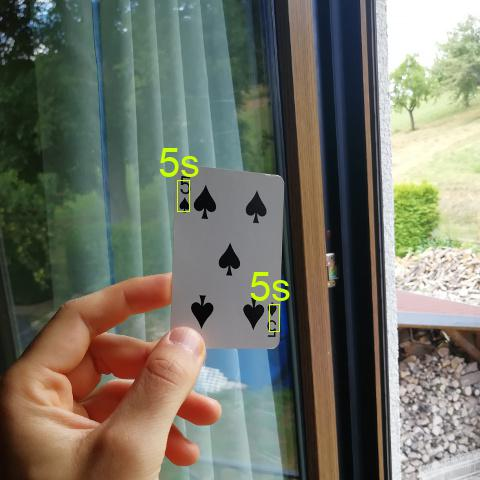
\includegraphics[width=44mm]{success3} &   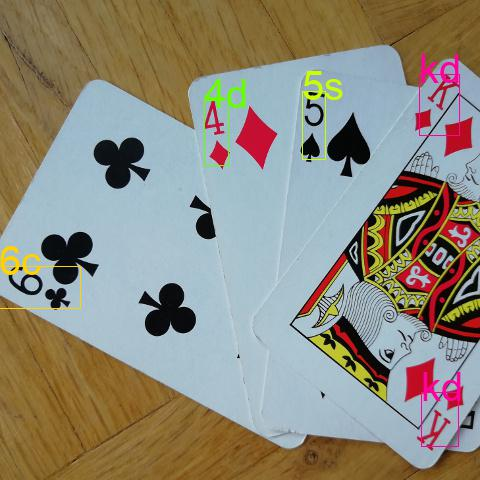
\includegraphics[width=44mm]{success2} &   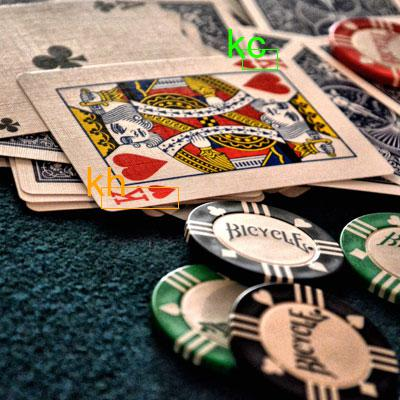
\includegraphics[width=44mm]{success1}\\
\makecell{\textbf{success:} scenario with a \\ highly diverse background}  & \makecell{\textbf{success:}  multiple cards \\ with trivial background} & \makecell{\textbf{success:}  angled shot of sheared card \\ in front of highly diverse background}\\[6pt]
  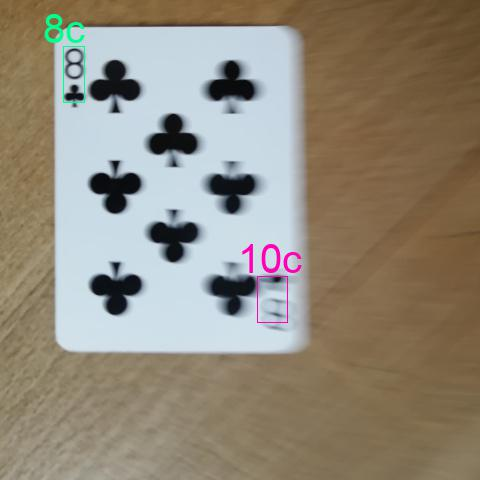
\includegraphics[width=44mm]{fail1} &   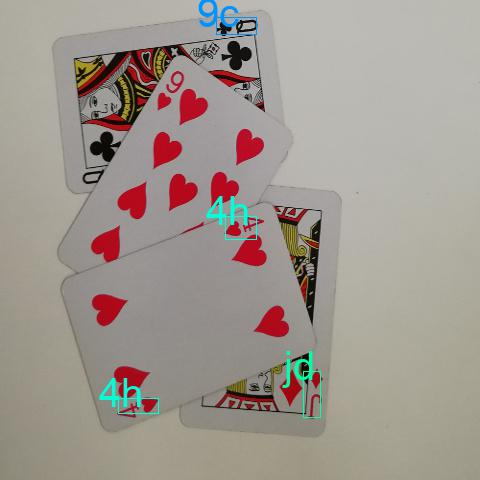
\includegraphics[width=44mm]{fail2} &   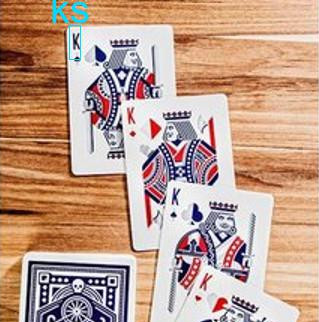
\includegraphics[width=44mm]{fail3}\\
\makecell{\textbf{fail:}  misdetection of 8c \\ due to motion blur} & \makecell{\textbf{fail:} misdetection of Qc and non- \\detection of 9h for unknown reason} & \makecell{\textbf{fail:} non-detection of Kd, Kh, Ks \\ due to wildly different distribution} \\[6pt]



\end{tabular}
\caption{Successful cases of detection (top row) and typical fail cases (bottom row) }
\end{figure}
As was to be expected, when multiple cards were present in an image, it was harder to find a rightfully classified image than to find one that our model did some mistakes on (middle column) as we trained on images with single cards only. Yet, in images with only one card, our model seems quite robust, at least if there is not too much blurring or other types of cluttering going on. Also, as we trained on a single deck of cards, it seems natural that the model has problems with predicting cards coming from completely different decks.
\subsection*{Extensions and tricks used in training}
\subsubsection*{Transfer learning}
For all experiments above, we started training using a network pre-trained on the VOC dataset (CITE). However, we also experimented with using our own fine-tuned weights from previous datasets for training. This generally led to distinctly faster convergence which makes sense as the distribution of weights for similar datasets will obviously be similar. However, this was not much of a concern as the training procedure was fast and further speed-ups were not needed.
\subsubsection*{Webcam deployment}
Depending on the scenery, our model running on a laptop webcam resulted in satisfactory to good results.
\section{Discussion and Future Work}
\subsection{Overview}
Using an artificially created annotated dataset of playing cards in situations reflecting realistic scenarios as good as possible, we perform object detection using the YOLOv3 object detection algorithm, achieving a mAP score of 97.30\% on a holdout dataset. \\ 
\subsubsection*{Training process}
The training procedure went rather swiftly. Apparently,  the particular task of detecting ranks/suits of playing cards is easy for our model - it can be thought of as 2D rather than 3D - in the end, playing cards are flat pieces of paper that do not show much variation in a 3D-world unlike other natural objects where algorithms have to learn representations of varying angle and shadow conditions or situations involving occlusion and the likes. \\
\subsubsection*{Deployment on a webcam}
Testing our model on a webcam resulted in satisfactory,  results. In many scenarios, especially with very bright backgrounds, the "black" suits \textit{clubs} and \textit{spades} dominated the scenery and were generally easier to be detected. We hypothesize two possible explanations for this: First, our dataset and corresonding transformations might not be general enough to cover the kinds of images captured by a stock laptop webcam. Second,   

\subsection{Future Work}
Our work works pretty well in the limited domain described above. However, if we were to develop a more reliable system, there are several extensions to be made.
\begin{description}
\item[more general dataset] The probably largest room for improval lies in the generation of a more general dataset - we trained on a single deck of cards, using one set of photographs. A more reliable approach would be to train on several decks of cards, include more than one card per image, use more actual photos of more realistic lighting situations, use realistic images as backgrounds instead of textures etc.
Also, we did not include the realistic scenario of shadows in the dataset at all, which also compromises generalisability.
\item[more thorough hyperparameter search] There are several hyperparameters of YOLO

\item[explore other architectures] Quite possibly, the inclusion of a more general dataset would cause tiny YOLOv3 to be overwhelmed. While such small architectures are beneficial to training times and risk of overfitting, they also encounter difficulties when relationships to be learned become overly complex. Especially including images with a very large scaling range introduces a large number of more stuff to be learned.
\item[cross-validation] We tested our model on a fixed set of test images. While there is nothing wrong with this approach, it also involves the risk of overfitting hyperparameters to this test set. A more thorough, yet more expensive approach would be repeatedly training models on different h.......... We made sure not to make parameters of our final model dependent on evaluation metrics of the test set, so this was not a big deal.
\end{description}
We did not include shadow and stuff
\section{Conclusion}
Using the YOLOv3 object detection algorithm, we managed to detect the suits and ranks of playing cards in a general setting. Hereby, our project served as a proof-of-concept - in order to build a model that is actually able to help people cheat effectively, several extensions would need to be made to our approach, which include... \\ Another issue to solving this is the lack of commodity contact lenses equipped with video cameras and GPUs in close proximity - until then, card game players will be protected from this kind of fraud.


\end{document}
